\documentclass[draft=false
              ,paper=a4
              ,twoside=false
              ,fontsize=11pt
              ,headsepline
              ,BCOR10mm
              ,DIV11
              ,bibtotoc
              ,liststotoc
              ]{scrbook}
\usepackage[ngerman,english]{babel}
%% see http://www.tex.ac.uk/cgi-bin/texfaq2html?label=uselmfonts
\usepackage[T1]{fontenc}
\usepackage[utf8]{inputenc}
%\usepackage[latin1]{inputenc}
\usepackage{libertine}
\usepackage{pifont}
\usepackage{microtype}
\usepackage{textcomp}
\usepackage[german,refpage]{nomencl}
\usepackage{setspace}
\usepackage{makeidx}
\usepackage{listings}
\usepackage{natbib}
\usepackage[ngerman,colorlinks=true]{hyperref}
\usepackage{soul}
%\usepackage{hawstyle}
\usepackage[printer]{hawstyle}

%% define some colors
\colorlet{BackgroundColor}{gray!20}
\colorlet{KeywordColor}{blue}
\colorlet{CommentColor}{black!60}
%% for tables
\colorlet{HeadColor}{gray!60}
\colorlet{Color1}{blue!10}
\colorlet{Color2}{white}

%% configure colors
\HAWifprinter{
  \colorlet{BackgroundColor}{gray!20}
  \colorlet{KeywordColor}{black}
  \colorlet{CommentColor}{gray}
  % for tables
  \colorlet{HeadColor}{gray!60}
  \colorlet{Color1}{gray!40}
  \colorlet{Color2}{white}
}{}
\lstset{%
  numbers=left,
  numberstyle=\tiny,
  stepnumber=1,
  numbersep=5pt,
  basicstyle=\ttfamily\small,
  keywordstyle=\color{KeywordColor}\bfseries,
  identifierstyle=\color{black},
  commentstyle=\color{CommentColor},
  backgroundcolor=\color{BackgroundColor},
  captionpos=b,
  fontadjust=true
}
\lstset{escapeinside={(*@}{@*)}, % used to enter latex code inside listings
        morekeywords={uint32_t, int32_t}
}
\ifpdfoutput{
  \hypersetup{bookmarksopen=false,bookmarksnumbered,linktocpage}
}{}

%% more fancy C++
\DeclareRobustCommand{\cxx}{C\raisebox{0.25ex}{{\scriptsize +\kern-0.25ex +}}}

\clubpenalty=10000
\widowpenalty=10000
\displaywidowpenalty=10000

% unknown hyphenations
\hyphenation{
}

%% recalculate text area
\typearea[current]{last}

\makeindex
\makenomenclature

\usepackage{graphicx}
\begin{document}
\selectlanguage{ngerman}

%%%%%
%% customize (see readme.pdf for supported values)
\HAWThesisProperties{Author={Corinna Klaukin}
	,Title={Modellierung und Visualisierung einer Population von Boids}
	,EnglishTitle={Modelling and Visualization of a Population of Boids}
	,ThesisType={Bachelorarbeit}
	,ExaminationType={Bachelorprüfung}
	,DegreeProgramme={Bachelor of Science Angewandte Informatik}
	,ThesisExperts={Prof. Dr. Philipp Jenke \and Prof. Dr. Stefan Sarstedt}
	,ReleaseDate={20. Oktober 2016}
}

%% title
\frontmatter

%% output title page
\maketitle

\onehalfspacing

%% add abstract pages
%% note: this is one command on multiple lines
\HAWAbstractPage
%% German abstract
{Schwarmverhalten, Boids, Populationssimulation, Künstliches Leben, Three.js, Javascript}%
{Das Thema dieser Arbeit ist die Simulation von Populationen von Schwarmtieren. Grundlage dafür ist das Boids-Modell, welches das lebensecht wirkende Schwärmen von digitalen Schwarmtieren ermöglicht. Dieses Modell wird in dieser Arbeit um einen Lebenszyklus, komplexe Verhaltensweisen und Genetik erweitert, um solche Schwärme als Populationen simulieren zu können. Ergebnis ist ein Prototyp, der mit Javascript und der 3D-Grafikbibliothek Three.js entwickelt wird und der das Populationsmodell implementiert und visualisiert.}
%% English abstract
{swarming behaviour, boids, simulation of a population, artificial life, Three.js, Javascript}%
{The topic of this thesis is the simulation of swarming populations. Basis for this is the boids model, which provides seemingly real swarming behaviour of digital swarm animals. In this thesis the boids model is being extended with a life cycle, complex behaviour and genetics, in order to simulate swarms as populations. The result is a prototype, written in Javascript and the 3d graphics library Three.js, which implements and visualizes the population model.}

\newpage
\singlespacing

\tableofcontents
\newpage
%% enable if these lists should be shown on their own page
\listoftables
\listoffigures
%\lstlistoflistings

%% main
\mainmatter
\onehalfspacing
%% write to the log/stdout
\typeout{===== File: chapter 1}
%% include chapter file (chapter1.tex)
%%\include{chapter1}

%%%%
\chapter{Einleitung}\label{einleitung}
\section{Motivation}
In der Computergrafik können bereits viele Naturphänomene simuliert werden, so auch das Schwarmverhalten von Schwarmtieren, wie Vögel und Fische.
Solche Simulationen wurden schon vielfach in Filmen und Animationen verwendet, wie z.B. in Batman Returns und Der König der Löwen \cite{movies}. Es gibt mittlerweile Modelle, einige performanter, andere dafür realistischer, die für solche Animationen eingesetzt werden. Eines der bekanntesten ist das Boids-Modell \cite{reynolds87}. In diesem Modell entscheidet jedes Tier anhand von festgelegten Regeln, wohin es sich bewegt. Doch dieses Modell, obwohl so einfach und naturnah, simuliert nur das pure Schwärmen. Eine ganzheitliche Sicht auf die Schwarmpopulation und den Lebenszyklus der Tiere ist bis jetzt nicht beachtet worden. In kurzen Filmsequenzen mag dies nicht weiter auffallen. Aber werden Schwarmsimulationen nach dem Boids-Modell in offenen Welten eingesetzt, in denen man nicht nur Zeit zum Erkunden, sondern auch zum Verweilen und Beobachten hat, so fällt schnell auf, dass die Tiere nur ein sehr limitiertes Verhaltensmuster zeigen.
Wenn in solchen Situationen Populationen von Schwarmtieren simuliert werden sollen, so ist ein ganzheitlicheres Modell vonnöten.

\section{Zielsetzung}
Ziel dieser Arbeit ist die Modellierung und Visualisierung einer Population von Boids.

Dabei soll im ersten Schritt das Modell der Boids von Craig Reynolds \cite{reynolds87} in seinen Grundzügen umgesetzt werden.

Der Schwerpunkt dieser Arbeit setzt auf die Entwicklung eines Populationsmodells, d.h. dass das Modell den Lebenszyklus der Boids darstellen soll. Dazu gehören eine begrenzte Lebensspanne, Bedürfnisse wie Hunger und Erschöpfung, die Paarungszeit und Bedrohung durch Fressfeinde.
Zu einer Population gehört außerdem Vererbung, so dass die Genetik der Boids zu modellieren ist.

Für das Modell soll ein Prototyp entwickelt werden, der eine Population von Boids mit einigen Erweiterungen geeignet visualisiert.
Dieser Prototyp beschränkt sich auf die korrekte Umsetzung des Modells und einer ansprechenden Visualisierung. Weder das Modell noch der Prototyp erheben Anspruch auf physikalische Korrektheit. Und obwohl das Modell sich stärker von der Natur inspirieren lässt, so haben die Boids nicht den Anspruch, eine wirklich existierende Tierart oder exakte biologische Vorgänge zu simulieren.

Letztlich soll das Modell anhand des Prototyps untersucht werden, wie geeignet es ist, um eine Schwarmpopulation mit populationstypischen Kriterien zu simulieren.

\section{Aufbau der Arbeit}
Ein Einstieg in die Thematik und die Aufgabenstellung befindet sich im Kapitel \ref{einleitung}.

Ein Überblick über das natürliche Schwarmverhalten von Tieren wird in Kapitel \ref{natur} beschrieben. Der Begriff Population sowie die wichtigsten Elemente einer Population werden erläutert. Außerdem werden hier die wichtigsten bzw. bekanntesten Modelle für die Simulation von Schwarmtieren gegenübergestellt. Ein Überblick über das originale Modell der Boids findet sich ebenfalls hier, gefolgt von den mathematischen Grundlagen des Boids-Modells.

Die wichtigsten bzw. bekanntesten Modelle für die Simulation von Schwarmtieren werden in Kapitel \ref{stand} gegenübergestellt. Ein Überblick über das originale Modell der Boids findet sich ebenfalls hier, gefolgt von den mathematischen Grundlagen des Boids-Modells.

In Kapitel \ref{modell} wird das Modell für die prototypische Umsetzung entworfen. Da das Boids-Modell bereits im vorherigen Kapitel beschrieben wurde, werden hier lediglich die Erweiterungen um populationstypische Elemente erläutert. Dazu gehören die Verhaltensweisen der einzelnen Tiere und der genetische Ansatz.

Das Kapitel \ref{umsetzung} behandelt anschließend die Umsetzung eines Prototyps des Modells. Hier werden unter anderem die Architektur der Umsetzung, die Datenstrukturen und die Algorithmen der Umsetzung beschrieben.

Anschließend erfolgt in Kapitel \ref{eval} die Evaluation des Prototyps nach populationstypischen Kriterien.

Eine Zusammenfassung der Ergebnisse und ein Ausblick auf weitere Entwicklungsmöglichkeiten werden abschließend in Kapitel \ref{fazit} beschrieben.

\chapter{Schwarmverhalten in der Natur und Populationsforschung}\label{natur}
Dieses Kapitel beschreibt verschiedene Beispiele von Schwarmverhalten in der Natur. Außerdem wird geklärt, was eine Population ist und welche Forschungsgebiete dazu gehören.
\section{Schwarmverhalten in der Natur}
Schwarmverhalten wird in der Natur bei ganz unterschiedlichen Populationen beobachtet. Ob es nun Vögel, Bienen, Schafe, Heuschrecken oder Heringe sind, Schwarmverhalten scheint für viele Tierarten von lebenswichtigem Nutzen zu sein.
Gemeinsam haben alle diese Populationen, dass sie in großen Zahlen auftreten, wie z.B. Flamingos, die mit bis zu einer Million Tieren zusammen schwärmen \cite{flamingo}.
In dieser großen Anzahl fliegen bzw. schwimmen bzw. bewegen sie sich fort, dicht an dicht, alle in einer gemeinsamen Geschwindigkeit und gleicher Richtung. Trotz der hohen Dichte sind Kollisionen dabei eher selten.

Bei einigen Schwarmpopulationen ist kein Anführer erkennbar. Stare z.B. richten sich dabei nur nach ihren dichtesten Schwarmnachbarn. Sie können bis zu sieben unterschiedliche Artgenossen erkennen und unterscheiden. Die Entfernung spielt dabei eine eher untergeordnete Rolle. Studien haben gezeigt, dass allein die topologische Dichte entscheidend ist, wobei Artgenossen, die seitlich eines Stares fliegen, eher zur Orientierung gewählt werden \cite{Camperi715}. Die Auswahl der dichtesten Nachbarn ist demnach anisotrop. So kann ein Star bis zu zwanzig Artgenossen in seinem Blickfeld haben, er orientiert sich aber nur an sieben von ihnen.

Andere Schwarmtiere haben Anführer, wie z.B. Ameisen und Bienen. Durch die Pheromone, die z.B. die Bienenkönigin aussendet, wissen die anderen Bienen im Bienenstock, was sie als Nächstes zu tun haben und welche Rolle sie im Bienenschwarm übernehmen sollen. Wenn es Zeit zur Futtersuche ist, so ziehen ein paar Kundschafterbienen morgens aus, um die Gegend zu erkunden. Sie sollen dabei nicht selber Futter sammeln, sondern nur die nächstliegende bzw. beste Futterstelle ausfindig machen \cite{bees}. Wo diese Futterstelle liegt, vermitteln die Kundschafterbienen nach ihrer Rückkehr durch den sogenannten Schwänzeltanz den Arbeiterbienen, die sich dann auf den Weg machen und das Futter sammeln. Die Bienen agieren zwar individuell, d.h. sie finden alleine (mit der Beschreibung der Kundschafterbienen) den Weg, werden aber trotzdem kontrolliert durch die Pheromone der Bienenkönigin.
Nur wenn es für die Königin Zeit wird auszuziehen, zeigen Bienenschärme ein echtes Schwarmverhalten, wie den Flug der Flamingos. Alle Bienen, die der Königin folgen, suchen die Nähe zu dieser und bilden so eine dichte Masse an Bienen. In großen Trauben hängen sie z.B. von Bäumen und warten, bis die Kundschafterbienen einen geeigneten Ort für das neue Zuhause gefunden haben. Sobald dies der Fall ist, fliegt der gesamte Schwarm dicht an dicht in einer Einheit zu dem neuen Platz.

Ein weiteres Merkmal von Schwarmtieren ist das homogene Erscheinungsbild. Heringe wissen zwar nicht, wie sie selber aussehen, sind aber seit ihrer Geburt auf das Erscheinungsbild ihrer Schwarmkollegen geprägt und suchen instinktiv Schutz in einem homogenen Schwarm. Dadurch, dass die anderen Heringe des Schwarms diesen Hering seinerseits auch als homogenen Schwarmnachbarn erkennen, wird er gut in den Schwarm integriert. Ein Clownfisch dagegen würde auch instinktiv den Schutz eines homogenen Schwarms in den Heringen erkennen und suchen, würde von den Heringen aber als artfremd erkannt und daraufhin ausgegrenzt werden. Der Clownfisch wäre in einem solchen artfremden Schwarm sehr leicht zu erkennen und hätte hier kaum Lebenschancen.

Das gesamte Leben spielt sich im Schwarm gemeinsam ab. Heuschrecken ziehen gemeinsam von einem Futterplatz zum nächsten. Flamingos brüten zur selben Zeit an einem gemeinsamen Ort \cite{flamingo}. Besonders in einer so bedrohlichen Situation wie dem Brüten am Boden, bietet das Auftreten im Schwarm die größten Überlebenschancen für den Schwarm. Durch die schier unendliche Anzahl der gleichzeitig brütenden Tiere bleiben trotz Fressfeinden noch genügend Tiere übrig, die die Population überleben lassen. Beobachtet wurde hierbei auch, dass Flamingos bis zu 140 km von ihrer Futterstelle entfernt brüten. Elterntiere ziehen dabei morgens zu der Futterstelle los, sammeln Futter und fliegen nicht selten erst am nächsten Tag wieder zu der Brutstelle zurück\cite{flamingo}. Dabei findet dieser Flug, wie alle anderen Tätigkeiten auch, in großer Anzahl als Schwarm statt.

\section{Populationsforschung}
Eine Population ist eine Gruppe von zusammenlebenden Individuen, die genetisch zu einer Art gehören und sich miteinander fortpflanzen \cite{genetik}.

Zu der Populationsforschung gehören u.a. die Fachgebiete der Populationsgenetik und der Populationsdynamik.
\subsection{Populationsgenetik}
Die genetische Zusammengehörigkeit wird in der Populationsgenetik erforscht. Es wird die genetische Vielfalt untersucht, d.h. welche Gene wie häufig insgesamt in welchen Ausprägungen vorkommen. Des Weiteren wird beobachtet, wie sich diese genetische Vielfalt über die Generationen hinweg verändert. Einige Populationen haben eine erstaunliche genetische Vielfalt, d.h. einen großen Genpool.

Andere Populationen haben hingegen einen eher kleinen Genpool und sind eher in Gefahr auszusterben, da eine einzige Krankheit, die ein Tier einer Art erfolgreich infiziert, es bei den anderen Tieren der Art genau so leicht haben wird \cite{genetik}. Andererseits kann dies aber auch bedeuten, dass die Tiere dieser Population hoch spezialisiert und deshalb gerade gut angepasst an ihren Lebensraum sind.
\subsection{Populationsdynamik}
Die Populationsdynamik beobachtet das Wachstum bzw. die Fluktuation einer Population. Sie untersucht Geburten- und Sterberaten. Eine Population, in der sich über einen längeren Zeitraum die Geburten- und Sterberaten ausgleichen und somit die Populationsgröße gleich bleibt, gilt als stabil.

Faktoren, die die Population beeinflussen sind u.a. Krankheiten, Abwanderungen, Gefahren durch Fressfeinde, Menge und Vielfalt von Nahrung und Umweltkatastrophen.

\chapter{Modelle der Schwarmsimulation}\label{stand}
Versuche, Schwarmverhalten mithilfe eines Computers darzustellen, gab es schon einige. Die wichtigsten davon werden zur Übersicht und zum Vergleich vorgestellt. Auch eine Übersicht des grundlegenden Modells der Boids und die mathematischen Grundlagen befinden sich in diesem Kapitel.
\section{Partikelsysteme}
Als einer der frühesten Versuche, Schwarmtiere mit einem Computer darzustellen, wurde ein Partikelsystem bemüht. Partikelsysteme besitzen eine Punktquelle, von der die fuzzy Objekte, Partikel, ausgesendet werden \cite{Reeves:1983:PST:357318.357320}. Diese Partikelsysteme können sehr performant sein, haben aber den Nachteil, dass realistische Schwärme nicht möglich sind. Partikel haben nur eine begrenzte Lebensdauer und auch ein sehr begrenztes Flugverhalten. Sie eignen sich gut für Feuer oder Nebel, sind aber nicht für die Interaktion untereinander konzipiert \cite{reynolds87}. Partikelsysteme eignen sich somit lediglich für eine sehr reduzierte Darstellung von Schwärmen, die keinen Anspruch an naturnahe Realität erheben.
\section{Schwarmbasierte Optimierungssysteme}
Schwarmbasierte Optimierungssysteme modellieren eine Gruppe von selbstständig agierenden Einheiten, genannt Agenten. Diese Agenten haben bestimmte Ziele oder ein spezifisches Problem zu lösen. Vielfach werden die Agenten als homogene Masse modelliert, d.h. alle Agenten sind gleichberechtigt und haben die gleichen Möglichkeiten. In einigen solchen Systemen werden die Agenten hierarchisch modelliert. Das Optimieren wird häufig durch die Kombination mit einem genetischen Algorithmus erreicht. Inspiration bieten die Suchstrategien von Schwarmpopulationen aus der Natur, wie z.B. der Bienen-Algorithmus \cite{citeulike:8377514}.

Ein weiteres Beispiel ist der Ant Colony Optimization Algorithmus \cite{ulster9737}. Hier wird das Verhalten von Ameisen nachgeahmt, den kürzesten Weg zwischen zwei Punkten zu suchen. Ein Phänomen der Natur stellt hier einen geschickten Optimierungsalgorithmus zur Verfügung. Ameisen, die auf der Suche nach Futter sind, hinterlassen eine Duftspur, anhand derer sie selber und andere Ameisen die Futterquelle wiederfinden können. Je mehr Ameisen einem bestimmten Weg folgen, desto stärker wird die Duftspur. Je stärker die Duftspur, desto vielversprechender erscheint der Weg, so dass immer mehr Ameisen diesen Weg wählen und somit die Duftspur immer weiter verstärken. Trotzdem entscheiden sich einige vereinzelte Ameisen immer wieder in unregelmäßigen Abständen ohne erkennbaren Grund, einen anderen oder völlig neuen Weg einzuschlagen. Die Hoffnung, eine noch ergiebigere Futterquelle oder einen kürzeren, schnelleren oder einfacheren Weg zu einer bereits bekannten Futterquelle zu finden, treibt diese abweichende Handlung voran. Der Ant Colony Optimization Algorithmus ist dabei diesen letzteren, explorierenden Ameisen nachempfunden. Entgegen der Natur wird dieser Algorithmus hierbei aber sehr verkürzt. Eine Population von zufällig generierten Agenten (Ameisen) wird gestartet, die alle zufällig neue Wege erkunden. Nach einem bestimmten Zeitraum wird der Erfolg eines jeden Agenten ausgewertet. Bei einem weiteren Zyklus des Algorithmus werden Kopien der im vorherigen Zyklus erfolgreichsten Agenten generiert, die ihrerseits wieder die Gegend erkunden. Nach einigen Durchläufen kann mithilfe dieses Algorithmus eine gute Approximation für einen kürzesten Weg gefunden werden.

Dieser Algorithmus wird gerne bei der Planung von Straßen eingesetzt. Schwarmbasierte Optimierungssysteme sind zwar durch das Naturphänomen der Schwarmtiere inspiriert, sind aber in erster Linie darauf beschränkt, mit ausgewählten Verhaltensweisen (Ameisen suchen einen kürzeren Weg.) ein nur periphär ähnliches Problem (Straßenverbindung zwischen zwei Städten) zu lösen. Die genetischen Algorithmen betrachten nur für das Problem wichtige Parameter, während der getaktete Lebenszyklus der Population der Agenten völlig unrealistisch ist. Für die Darstellung eines Schwarmes allein um des Schwärmens Willen eignet sich dieser Ansatz also keinesfalls, obwohl die genetischen Algorithmen Ansätze bieten.
\section{Artificial Life und Behavioural Animation}
Der Bereich Artificial Life versucht, möglicht realistisch und lebensecht wirkende digitale Einheiten zu schaffen, die scheinbar eigenständig und ungesteuert ein eigenes Leben führen. Hierbei wird nicht selten die Natur als Vorbild genommen und versucht, diese nachzubilden, wie z.B. die Simulation eines Aquariums, in dem Fische zufällig und in nicht erkennbaren Zyklen das digitale Aquarium erkunden. Ein komplexeres Beispiel ist das Computerspiel Creatures \cite{norns}. In der künstlichen Welt Albia leben u.a. die Norns, die eigenständig die Welt erkunden, Hunger, Schmerz und Einsamkeit empfinden, mit Artgenossen kommunizieren und sich fortpflanzen. Besonders bemerkenswert ist hier die Komplexität der Norn-DNS.

Der Bereich Behavioural Animation nutzt Ansätze des Artificial Life, um möglichst echt wirkende Animationen zu erstellen \cite{reynolds87}. Die Jagd eines gefährlichen Haies auf den Wassermann Duffy wurde auf diese Weise generiert \cite{Funge:1999:CMK:311535.311538}. Sowohl Duffy als auch der Hai besaßen vorprogrammierte Verhaltensvorschriften und Bedürfnisse. Die genauen Einzelheiten der Jagd waren aber ungescriptet und sind durch Zufall entstanden.
Eine Simulation eines Schwarms in einem erweiterbaren Szenario im Hinsicht auf realitätsnahe Lebenszyklen im Populationsgedanken ist sicherlich hier denkbar.
\section{Boids-Modell nach Reynolds}
Der Erfinder der Boids, Craig Reynolds, hat sich intensiv mit Artificial Life und Behavioural Animation beschäftigt und dort auch seine Inspiration für die Boids geholt.
Das von ihm in den 1980er-Jahren entwickelte Modell der Boids \cite{reynolds87}\cite{oai:CiteSeerPSU:509294}\cite{Reynolds:1988:NBI} bezweckt die Simulation von einem Naturphänomen und folgt einer verhaltensbiologischen Theorie: Es wurde in der Natur beobachtet, wie sich Schwärme verhalten. Man hat gemutmaßt, dass das Verhalten auf einem einfachen Satz von Verhaltensregeln beruht. Da dieses Modell digitale künstliche Einheiten mit genau diesen Regeln dazu veranlassen kann, realitätsnahes Schwarmverhalten zu simulieren, wird die Theorie plausibel.

\begin{figure}[!h]
\centering
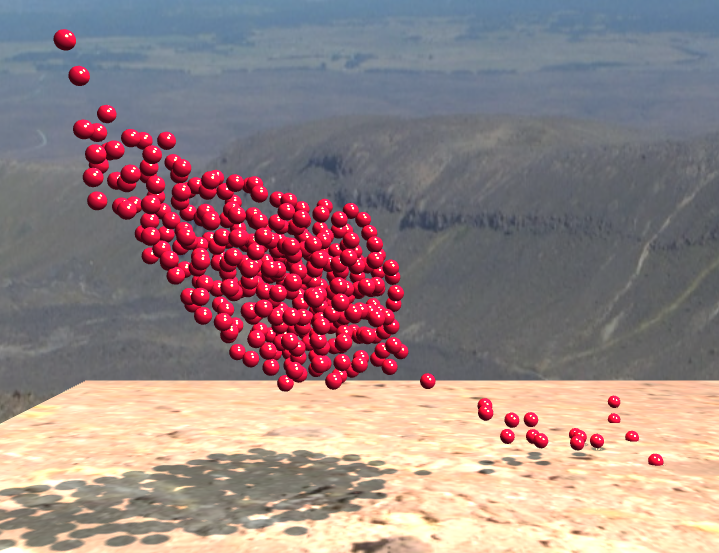
\includegraphics[scale=0.4]{project/bigswarm.png}
\caption{Schwärmende Boids}
\label{simple}
\end{figure}

Später wurde dieses Modell von Reynolds erweitert, um Hindernisse zu umgehen \cite{alife92*327}, eine Gruppe durch Korridore zu leiten \cite{reynolds:1994:ecfbnw} und die Parameter mithilfe von genetischen Algorithmen zu optimieren \cite{sab92:reynolds}. In dieser Arbeit wird aber nur die einfache Variante des Boids-Modells verwendet.

Die Grundregeln des Boids-Modells sind: Bleibe dicht bei deinen Artgenossen, passe dich in Geschwindigkeit und Ausrichtung an deine Artgenossen an und versuche, dich in den Mittelpunkt des Schwarms zu bewegen.
Es beinhaltet auch die Regel, einen Mindestabstand zu den Artgenossen einzuhalten.

Wie in der Abbildung \ref{simple} zu sehen ist, bestimmen diese wenigen Regeln ein erstaunlich realitätsnahes Verhalten, welches für viele Simulationen, in denen es genügt, den Schwarm endlos in der Luft fliegen zu lassen, völlig ausreicht. Dieses Grundregelwerk lässt sich sowohl im 2D- als auch im 3D-Raum durch einfache Vektorrechnung verwirklichen. Die bestimmenden Einflüsse auf die nächste Handlung eines Boids wird im Folgenden genauer beschrieben.
\subsection{Kohäsion (cohesion)}
Die Kohäsion ist die erste und wichtigste Regel, die für den Zusammenhalt eines Schwarms verantwortlich ist. Kohäsion bedeutet, dass alle Boids das Bedürfnis haben, dicht bei ihrem Schwarm zu bleiben. Der sicherste Platz in einem Schwarm ist dabei der Mittelpunkt, da Gefahren, wie z.B. ein Fressfeind, von den weiter außen fliegenden Boids abgeschirmt werden. Abbildung \ref{cohesion} zeigt das Bedürfnis eines Boids, möglichst in die Mitte des Schwarms zu gelangen.

\begin{figure}[!h]
\centering
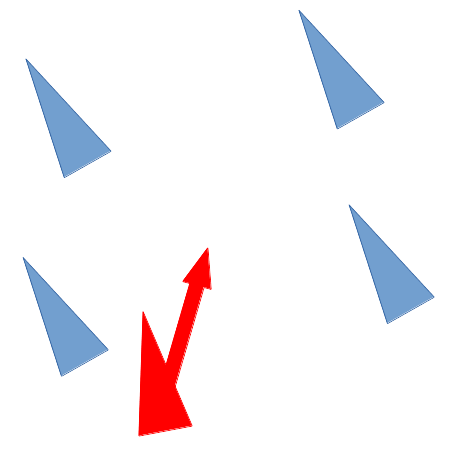
\includegraphics[scale=0.4]{project/cohesion.png}
\caption{Kohäsion nach Reynolds \cite{reynolds87}}
\label{cohesion}
\end{figure}

\subsection{Anpassen der Geschwindigkeit und Ausrichtung (alignment)}
Damit der Schwarm den Zusammenhalt und gemeinsame Flugmanöver gewährleisten kann, müssen sich die Boids an Geschwindigkeit und Ausrichtung der Schwarmnachbarn anpassen. Je schneller die Boids auf Änderungen reagieren, desto besser ist der Zusammenhalt. Reagieren die einzelnen Tiere nicht schnell genug oder passen sich nicht an, würde der Schwarm aufbrechen und fragmentieren. Ein einzelner Boid behält dabei seine dichtesten Schwarmnachbarn im Blickfeld und passt sich an diese an, wie in Abbildung \ref{alignment} zu sehen ist. Ändern sich die Nachbarn, bzw. gibt es Verschiebungen, die dazu führen, dass Nachbarn sich zum Vorteil anderer entfernen, so erkennt der Boid nun diese neuen, dichteren Boids als die nächsten Nachbarn an.

\begin{figure}[!h]
\centering
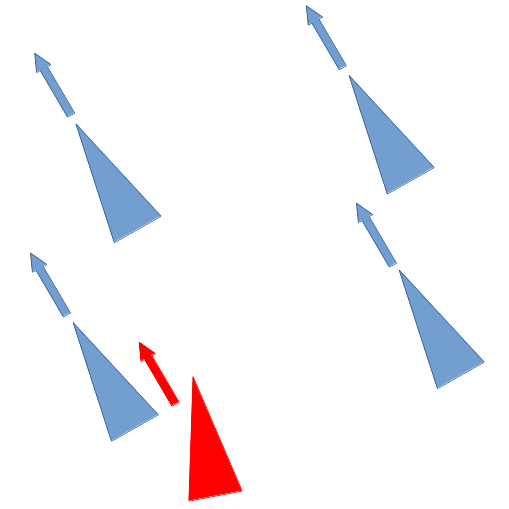
\includegraphics[scale=0.4]{project/alignment.png}
\caption{Anpassen in Geschwindigkeit und Ausrichtung nach Reynolds \cite{reynolds87}}
\label{alignment}
\end{figure}

\subsection{Mindestabstand (separation)}
Um nicht während des Schwärmens zu kollidieren und bei einer Richtungs- bzw. Geschwindigkeitsänderung der Schwarmnachbarn genügend Zeit und Raum zu haben, um auf die Änderungen zu reagieren, muss ein gewisser Mindestabstand gewährleistet werden. Dieser Mindestabstand darf aber nicht zu groß sein. Je dichter die Schwarmtiere zusammen fliegen, desto schwieriger ist es für einen Außenstehenden, wie z.B. einen Fressfeind, einzelne Boids zu erkennen und zu verfolgen. Die Abbildung \ref{separation} zeigt einen Boid, der zu dicht an einen seiner Nachbarn gekommen ist und deshalb wieder ein wenig zurück steuern muss.

\begin{figure}[!h]
\centering
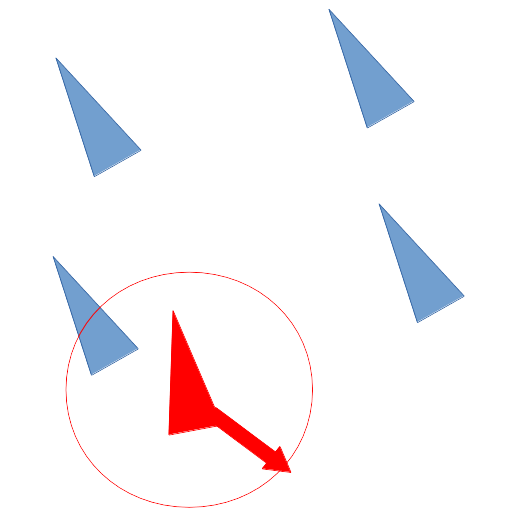
\includegraphics[scale=0.4]{project/separation.png}
\caption{Mindestabstand nach Reynolds \cite{reynolds87}}
\label{separation}
\end{figure}

\section{Mathematische Grundlagen des Boids-Modells}\label{mathe}
Für die Berechnung der Fortbewegung eines Boids kommt die Vektorrechnung zum Einsatz. Ein Grundverständnis für die Vektorrechnung wird vorausgesetzt und deshalb nicht weiter erläutert. Die Berechnungen sind die, die in dem Prototyp umgesetzt werden, und basieren grob auf anderen Implementationen \cite{Bourg:2004:AGD:1096109}\cite{nature}.

Ein Boid besitzt zum Zeitpunkt \(t_0\) die Position \(\vec{p}_0\) und die Velocity (den Bewegungsvektor) \(\vec{v}_0\). Die Position ist dabei ein Ortsvektor und die Velocity ein Richtungsvektor, der die Ausrichtung anzeigt. Die Länge der Velocity beschreibt die Geschwindigkeit.

Die nächste Position \(\vec{p}_1\) zum Zeitpunkt \(t_1\) ergibt sich durch das Addieren der neu zu berechnenden Velocity \(\vec{v}_1\) zu der aktuellen Position \(\vec{p}_0\).
\[\vec{p}_1 = \vec{p}_0 + \vec{v}_1 \]
Die neue Velocity \(\vec{v}_1\) zum Zeitpunkt \(t_1\) ergibt sich aus der Summe der aktuellen Velocity \(\vec{v}_0\) und der Beschleunigung, die sich aus den gemittelten Faktoren, die die Bewegung der Boids beeinflussen, berechnen lässt: Kohäsion \(\vec{coh}\), Anpassung an Geschwindigkeit und Ausrichtung \(\vec{ali}\) sowie Mindestabstand \(\vec{sep}\).
\[\vec{v}_1 = \vec{v}_0 + (\vec{coh}_1 + \vec{ali}_1 + \vec{sep}_1)\]

Da ein Boid nicht unendlich schnell beschleunigen kann, muss bei der Berechnung sichergestellt werden, dass die maximale Beschleunigung nicht überschritten wird.

Um die Beschleunigungsfaktoren priorisieren zu können, müssen sie gewichtet werden. Dabei muss sichergestellt sein, dass jeder einzelne Faktor die maximale Beschleunigung nicht überschreitet, damit die Priorisierung allein durch die Gewichte \(w\) getragen wird.

Daraus ergibt sich nun für die Berechnung der Position die folgende Formel:
\[\vec{p}_1 = \vec{p}_0 + \vec{v}_0 + w_{coh} * \vec{coh}_1 + w_{ali} * \vec{ali}_1 + w_{sep} * \vec{sep}_1\]

\subsection{Berechnung der Kohäsion}
Der Kohäsionsvektor \(\vec{coh}_1\) ist der Vektor, der den Boid in das Zentrum des Schwarms \(\vec{z}_1\) lenkt. Das Zentrum des Schwarms \(\vec{z}_1\) ist die gemittelte Summe der Positionen aller Boids \(\vec{pos}_n\).

\[\vec{z}_1 = \frac{\sum \limits_{n=0}^n \vec{pos}_n}{n} \]
Von der aktuellen Position \(\vec{p}_0\) zu dem Zentrum \(\vec{z}_1\) ergibt sich der Vektor \(\vec{p}_0\vec{z}_1\) folgendermaßen:
\[\vec{p}_0\vec{z}_1 = \vec{z}_1 - \vec{p}_0\]
Nach Einsetzen von \(\vec{p}_0\) ergibt sich daraus:
\[\vec{p}_0\vec{z}_1 = \frac{\sum \limits_{n=0}^n \vec{pos}_n}{n} - \vec{p}_0\]
Da ein Boid nur eine begrenzte Geschwindigkeit besitzt, aber dennoch den Kohäsionspunkt maximal anstreben soll, wird der Kohäsionsvektor \(\vec{coh}_1\) auf die Höchstgeschwindigkeit gesetzt, indem \(\vec{p}_0\vec{z}_1\) normalisiert und dann mit der Höchstgeschwindigkeit des Boids multipliziert wird.
\[\vec{coh}_1 = \frac{\vec{p}_0\vec{z}_1}{|\vec{p}_0\vec{z}_1|} * maxspeed\]
Um eine sanfte Kurve zu fliegen, muss \(\vec{coh}_1\) mit der Velocity \(\vec{v}_0\) gemittelt werden.
\[\vec{coh}_1 = \frac{\vec{p}_0\vec{z}_1}{|\vec{p}_0\vec{z}_1|} * maxspeed - \vec{v}_0\]

\subsection{Berechnung der Ausrichtung und Geschwindigkeit}
Der Vektor \(\vec{ali}_1\), der den Boid in Ausrichtung und Geschwindigkeit anpasst, berechnet sich ähnlich wie der Kohäsionsvektor \(\vec{coh}_1\). Die gemittelte Velocity \(\vec{v}_{gem}\) der Boids wird normalisiert, auf die Höchstgeschwindigkeit gesetzt und mit der aktuellen Velocity \(\vec{v}_0\) gemittelt.
\[\vec{v}_{gem} = \frac{\sum \limits_{n=0}^n \vec{v}_n}{n}\]
\[\vec{ali}_1 = \frac{\vec{v}_{gem}}{|\vec{v}_{gem}|} * maxspeed - \vec{v}_0\]

\subsection{Berechnung des Mindestabstandes}
Der Vektor \(\vec{sep}_1\), der für den Einhalt des Mindestabstandes des Boids sorgt, kommt nur zum Tragen, wenn der Mindestabstand zu mindestens einem benachbarten Boid verletzt wird. Ansonsten bleibt dieser Vektor ein Nullvektor. Die Distanz \(d\) zwischen der Position \(\vec{p}_0\) und der des Nachbarn \(\vec{pos}\) ist die Länge des Vektors \(\vec{p}_0\vec{pos}\), also \(d = |\vec{p}_0\vec{pos}|\).

Bei der Berechnung des Vektors \(\vec{sep}_1\) kann man sich die Berechnung des Kohäsionsvektors \(\vec{coh}_1\) zu Nutze machen, in dem man das Zentrum der Positionen der zu dicht fliegenden Nachbarn \(\vec{pm}_1\) mit dem Zentrum des Schwarms \(\vec{z}_1\) gleichsetzt. Dies würde den Kollisionsweg des Boids mit den Nachbarn berechnen. Da das ja gerade nicht gewollt ist, wird das Ergebnis umgekehrt, so dass nun der Weg zur Kollisionsvermeidung ermittelt wird.
\[\vec{p}_0\vec{pm}_1 = \frac{\sum \limits_{n=0}^n \vec{pos}_n}{n} - \vec{p}_0\]
\[\vec{sep}_1 = \vec{v}_0 - \frac{\vec{p}_0\vec{pm}_1}{|\vec{p}_0\vec{pm}_1|} * maxspeed\]

\chapter{Entwurf des Populationsmodells}\label{modell}
Nachdem im vorherigen Kapitel eine Beschreibung des Boids-Modells zu finden war, wird in diesem Kapitel beschrieben, welche Anforderungen der Populationsgedanke an ein erweitertes Modell hat. Dazu gehören zusätzliche Bedürfnisse der einzelnen Boids, wie z.B. Hunger, aber auch eine Modellierung der Genetik und des Lebenszyklus der Boids. Da sich daraus für den Boid mehrere mögliche Handlungen zu einem jeden Zeitpunkt ergeben, wird im Nachhinein die Priorisierung und Entscheidungsfindung erläutert.
\section{Das pure Schwärmen}
Das Boids-Modell in seiner ursprünglichen Version wird in seinen Grundzügen für das reine Schwärmen übernommen. Die einzelnen Boids orientieren sich an ihren direkten Nachbarn und passen sich in Geschwindigkeit und Richtung an, wahren einen Mindestabstand und suchen die Mitte des Schwarms.
\subsection{Performanz}\label{lahm}
So einfach der Schwarmalgorithmus auch ist, so gibt es jedoch ein Performanzproblem bei einer größeren Anzahl von Boids: Nach dem ursprünglichen Algorithmus fragt jeder Boid jeden anderen nach Position, Geschwindigkeit usw. Es liegt also eine Komplexität O(n²) vor \cite{reynolds87}. Bei einer kleinen Population von nur 20 Boids, wie in diesem Prototyp gewählt, gibt es bei dem Algorithmus bereits 400 Abfragen. Bei realistischen Populationsgrößen, wie in einigen Flamingoschwärmen zu finden, müsste man von einer Million Tieren ausgehen. Trotz Verbesserungen der Prozessoren ist es noch nicht möglich, solche Schwärme in Echtzeit zu simulieren. Selbst bei kleineren Schwärmen von nur 4000 Tieren ist die nötige Rechenleistung beträchtlich.

Zur Verbesserung der Performanz muss deshalb der Algorithmus verbessert werden. Ein Ansatz ist die Beschränkung der Orientierung auf die direkten Nachbarn. Hier ist sogar die Natur das Vorbild: Wie bereits in Kapitel \ref{natur} erwähnt, orientieren Stare sich in der Natur auch nicht an allen anderen Tieren im Schwarm, sondern nur an bis zu sieben der dichtesten Nachbarn. Die Komplexität dieser Lösung wäre statt O(n²) nur noch O(7n). Bei kleineren Populationen wie in diesem Prototyp ist der Unterschied noch nicht sehr groß, aber wie die Tabelle \ref{komplexitaet} zeigt, profitieren Umsetzungen mit großen Populationen beträchtlich.

\begin{table}[h]
\centering
\begin{tabular}{c|c|c}
	Populationsgröße & jeder fragt jeden & Reduzierung der dichtesten Nachbarn\\
	\hline
	20 & 400 & 140\\
	100 & 10 000 & 700\\
	4000 & 16 Millionen & 28 000\\
	1 Million & 1 Billion & 7 Millionen\\
\end{tabular}
\caption{Komplexität des Schwarmalgorithmus gemessen anhand von Abfragen der Positionen der Artgenossen}
\label{komplexitaet}
\end{table}

Dennoch sind in dem erweiterten Populationsmodell mehrere Iterationen über die gesamte Population nötig, um die Werte der Boids zu überwachen und anzupassen. Eine Möglichkeit, den Rechenaufwand zu verringern, ist es, solche Updates in langsamer getakteten Abständen durchzuführen.
\subsection{Sichtbarkeit}
Wie soeben beschrieben sollte aus Performanzgründen die Sichtbarkeit der Boids beschränkt werden. Auch Beispiele aus der Natur legen dies nahe, wie bereits in Kapitel \ref{natur} beschrieben. Es ist bei der Anpassung der Ausrichtung und der Geschwindigkeit also die Auswahl auf die direkten Nachbarn zu beschränken. Eine Möglichkeit ist die Nutzung der Datenstruktur des Schwarms: Ein Octree kann üblicherweise auf Anfrage alle Elemente in einem gesuchten Radius finden. Da der Octree bereits als Datenstruktur gewählt wurde, bestärkt dies den Einsatz des Octrees in diesem Prototyp.
\section{Erweiterung der Verhaltensweisen}
Der originale Ansatz von Reynolds ist noch sehr einfach. Wie in der Natur kann ein Außenstehender die einzelnen Boids nicht unterscheiden. Auch das Modell von Reynolds behandelt sie wie anonyme, austauschbare Einheiten. Die Boids haben keine Identität, keine Eigenschaften, nur eine Position. Das Modell jedoch, welches in dieser Arbeit entwickelt wird, soll die Boids realistischer darstellen. Um eine komplexere Handlungskette zu modellieren, werden Informationen zu vergangenen Handlungen und veränderbaren Zuständen zwingend erforderlich. Dazu gehören die jeweilige DNS, das aktuelle Bedürfnis und daraufhin eben eine Identität. Die Boids in diesem System sind nicht austauschbar und deutlich komplexer.
\subsection{Futtersuche und Ruhepausen}
Alle Lebewesen dieser Welt benötigen zum Leben Energie, die sie durch die Aufnahme von Nahrung gewährleisten. Aufgenommene Energie wird vom Organismus aufgebraucht, so dass nach gewisser Zeit für Nachschub gesorgt werden muss. Ist nicht genug Nahrung vorhanden, reicht die gespeicherte Energie nicht aus, so verstirbt der Organismus. Zur Verwertung von Nahrung und deren Umwandlung in Energie sind des Weiteren Ruhepausen notwendig. Dieses grundlegende Prinzip des Lebens darf bei der Modellierung einer Population auf gar keinen Fall fehlen.

Das neue Modell beinhaltet den aktuellen Status der Energie- bzw. Hungerlevel. Des Weiteren wird die Information über die maximale Energiekapazität benötigt. Zur Laufzeit des Systems muss in regelmäßigen Abständen der aktuelle Hunger- und Müdigkeitslevel realitätsnah angepasst werden: Bei energieverbrauchenden Aktivitäten wie Fliegen sinken die Energiewerte, bei Nahrungsaufnahme und Ruhepausen steigen sie. Damit die Boids dem Schwärmen-Futtersuche-Zyklus folgen können, müssen sie Hunger und Müdigkeit erkennen können. Dies kann mithilfe von Schwellwerten ermittelt werden. Durch Überwachung der Energie- und Schwellwerte kann ein Boid erkennen, wann die Energiewerte zu niedrig werden und der Nachschub von Energie in Form von Nahrung wichtig wird. Ist das der Fall, wird es für einen Boid zunehmend wichtiger, eine Nahrungsquelle ausfindig zu machen. Das Bedürfnis, dicht bei den schwärmenden Artgenossen zu sein, wird dabei momentan geringer.


\begin{figure}[htp]
\centering
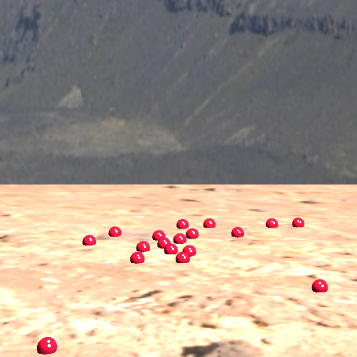
\includegraphics[scale=0.50]{project/ground.png}
\caption{Boids suchen nach Nahrung}
\label{onground}
\end{figure}

Ist ein Boid wie in der Abbildung \ref{onground} am Boden, frisst und ruht sich aus, so genügt es nicht zu warten, bis die Energiewerte den Schwellwert wieder positiv überschreiten, sondern ein Boid kehrt erst wieder zum Schwärmen zurück, wenn seine Sättigung bzw. Erholung das Energiemaximum erreicht.
Abschließend darf man nicht vergessen, sich zu fragen, was passiert, wenn die Energielevel auf null sinken, bevor der Boid die Chance hat, neue Nahrung zu finden. Genau wie für echte Organismen auch bedeutet dies für die Boids den Tod durch Erschöpfung oder Verhungern.
\subsection{Abwehr der Fressfeinde}\label{enemy}
Eine weitere Gefahr für Schwarmtiere stellen Fressfeinde dar: Heringe können einem Hai zum Opfer fallen, Ameisen können von Amseln gefressen werden. Normalerweise haben Schwarmtiere keine guten Chancen, sich aktiv zu verteidigen.

Eine Strategie ist der dichte Zusammenhalt: Die Masse und das homogene Erscheinungsbild der Schwarmtiere macht es Angreifern schwer, einzelne Tiere zu erkennen und zu verfolgen. Diese Strategie wird von dem originalen Ansatz des Modells bereits sehr gut erfüllt.

Die zweite Strategie zur Abwehr ist die Flucht. Wenn ein Angreifer erkannt wird und zu nahe kommt, dann ist es dem Boid geraten, schnell darauf zu reagieren und so schnell wie möglich vor dem Angreifer zu fliehen. Dies erfordert die Intelligenz, Angreifer als solche zu erkennen. In einem digitalen Computermodell gibt es natürlich keine Angreifer, die nicht vorsätzlich modelliert wurden. Eine einfache Möglichkeit, die Erkennung von Angreifern zu modellieren, ist, den Boids eine Liste von Angreifern zugänglich zu machen. Dann kann ein Boid in jedem Update-Zyklus die aktuelle Position der Angreifer ermitteln und bei der Unterschreitung einer Minimaldistanz die Entscheidung zur Flucht fällen.

Sehr realistisch ist diese Variante aber nicht. Gerade in der Mitte des Schwarms hat ein Boid nur seine Artgenossen im Blickfeld. Und das Wissen um alle in der Welt vorkommenden Fressfeinde und deren Position ist echten Schwarmtieren auch nicht vergönnt.
Eine bessere Variante wäre es, einen Angreifer erst zu erkennen, wenn er im Sichtfeld des Boids auftaucht. Dies wäre mithilfe von Rays, die vom einzelnen Boid ausgehen und eine festgelegte Länge aufweisen, machbar. Wenn ein Ray mit einem Angreifer kollidiert, dann ist offensichtlich die Flucht vonnöten.

Eine dritte und für die Boids wohl realistischste Variante wäre, für jeden Boid das Sichtfeld aus seiner Perspektive zu berechnen und mit Bildverarbeitung und intelligenten Methoden, wie z.B. Neuronalen Netzen, nach Angreifern zu durchsuchen.

Bei der Auswahl der Varianten ist zwischen deren Komplexität, Performanzansprüchen und Realitätsnähe abzuwägen. Für eine Simulation ändert sich augenscheinlich nichts, da nur die Erkennung der Angreifer unterschiedlich wäre, aber nicht die Handlung der Boids. Für diese Arbeit wurde die erste Variante als die beste empfunden, da sie die naheliegendste und einfachste ist.

\section{Evolution}
Eine Population, die nie neue Mitglieder erhält, stirbt früher oder später aus. Damit die Population überleben kann, muss also für Nachschub gesorgt werden. Das Erzeugen von Nachkommen ist in der Natur vielfältig und bei jeder Tierart anders. Bei Flamingos finden sich ein weibliches und ein männliches Tier und brüten Eier aus. Viele Vogelarten zeigen ein solches partnerschaftliches Verhalten. Dies ist auch der Ansatz, der für dieses Modell gewählt und im Folgenden näher beschrieben wird.

\subsection{Genetik}
Die biologische Genetik ist ein sehr komplexes und faszinierendes Thema, wird in dieser Arbeit aber nur sehr oberflächlich abgehandelt. Ein tieferer Einstieg in diese Thematik würde den Rahmen sprengen und das Modell unnötig verkomplizieren. Exakte genetische Vorgänge \cite{genetik} sind für eine Simulation zu komplex und bieten zu wenig Mehrwert. Im Folgenden wird ein sehr vereinfachtes Modell entwickelt.

\begin{figure}[!h]
\centering
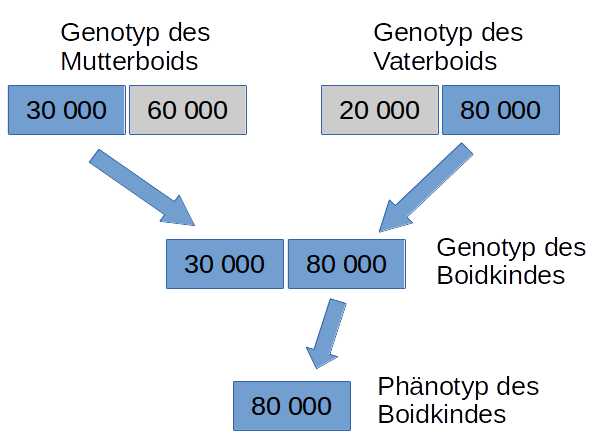
\includegraphics[scale=0.30]{project/rekombination.png}
\caption{Rekombination am Beispiel der Lebensspanne}
\label{rekombination}
\end{figure}

Gene sind die genetischen Faktoren, die dafür verantwortlich sind, dass Merkmale ausgeprägt werden. Diese werden bei der Fortpflanzung an die Nachfahren vererbt. Bei der geschlechtlichen Vererbung wird zufällig entschieden, welche der genetischen Informationen vom Mutter- und Vatertier an den jeweiligen Nachkommen weitergegeben wird. Dieser Vorgang nennt sich Rekombination und wird in Abbildung \ref{rekombination} visualisiert. Das genetische Erbmaterial nennt sich Genotyp und repräsentiert seine exakte genetische Ausstattung. Die Informationen, die sich bei dem Individuum durchsetzen, werden im Phänotyp beschrieben.

Jeder Boid hat demnach einen Genotyp, in dem die vererbten Gene, wie z.B. die maximale Lebensdauer und maximale Fluggeschwindigkeit, gespeichert werden. Zu jedem Gen sind zwei Optionen vorhanden, eine vom Vatertier, die andere vom Muttertier. Welche Information sich durchsetzt und damit im Phänotyp gelistet wird, ist zufällig. Weist z.B. das Erbgut die mögliche Lebensspanne des Vaters und die der Mutter auf, wird für den Phänotyp per Zufall die Lebensspanne des Vaters ausgewählt. Dies ist demnach die für das Boidkind geltende maximal zu erreichende Lebensspanne wie in Abbildung \ref{rekombination} zu sehen ist.

Die initiale Generation wird per Zufall generiert. Ab dann werden neue Nachkommen durch Rekombination erzeugt. Dazu werden die Erbinformationen der Elterntiere, d.h. die Genotypen, neu kombiniert und an den Nachkommen vererbt. Daraus ergibt sich für den Nachkommen dann auch der neue Phänotyp.

\subsection{Partnersuche und Brüten}
Damit sich zwei Boids unterschiedlichen Geschlechts verpaaren können, müssen sie sich als solche erkennen und finden. Die Tiere in diesem Modell sind nicht monogam, sondern suchen sich in jeder Brutzeit neue Partner, in der Hoffnung, die genetische Varianz der Population zu erhalten.
Viele Tiere verpaaren sich nur zu bestimmten Zeiten: der Paarungszeit. Dazu muss das Modell in regelmäßigen Abständen eine solche verkünden, in der die Boids für den Fortbestand sorgen können.
Eine Variante, den geeigneten Partner zu finden, ist es, in der Paarungszeit den Boden aufzusuchen und unter den dort verweilenden Artgenossen einen geeigneten Partner auszuwählen. Haben sich zwei gefunden, gibt es Nachwuchs. Der Nachwuchs ist sofort flügge und die Elterntiere sind frei, sich am Boden neue Partner zu suchen, solange die Paarungszeit anhält.
Eine zweite, realistischere Variante wäre, Eier zu generieren, die abwechselnd von den Elterntieren bebrütet werden, während das andere Elterntier Futter sucht. Beide Elterntiere wären somit an das Nest gekoppelt und müssten evtl. die ausgeschlüpften Küken versorgen. Diese Variante modelliert sich enger nach dem natürlichen Verhalten von Schwarmvögeln.

Viele Tiere verpaaren sich erst, wenn sie alt genug sind bzw. die Geschlechtsreife erlangen. Das Modell muss demnach bei der Partnersuche streng überprüfen, wer an der Paarungszeit teilnimmt, so dass Jungtiere den adulten Tieren nicht als Partner zur Verfügung stehen.

\section{Entscheidungsfindung}
Die Entscheidung, welche Handlung der Boid als Nächstes zu verfolgen hat, ergibt sich aus den aktuellen Werten (z.B. Hungerlevel) und dem aktuellen Status (Schwärmen, Partner suchen...). Im ersten Schritt wird die Population überprüft: Alte, erschöpfte Tiere werden aussortiert, Nachkommen werden erzeugt.

Im zweiten Schritt werden die Werte der einzelnen Tiere überprüft und angepasst. Ist der Boid in der Luft am Schwärmen, werden die Energielevel gesenkt. Ist der Boid am Boden, steigen sie.

\begin{figure}[!h]
\centering
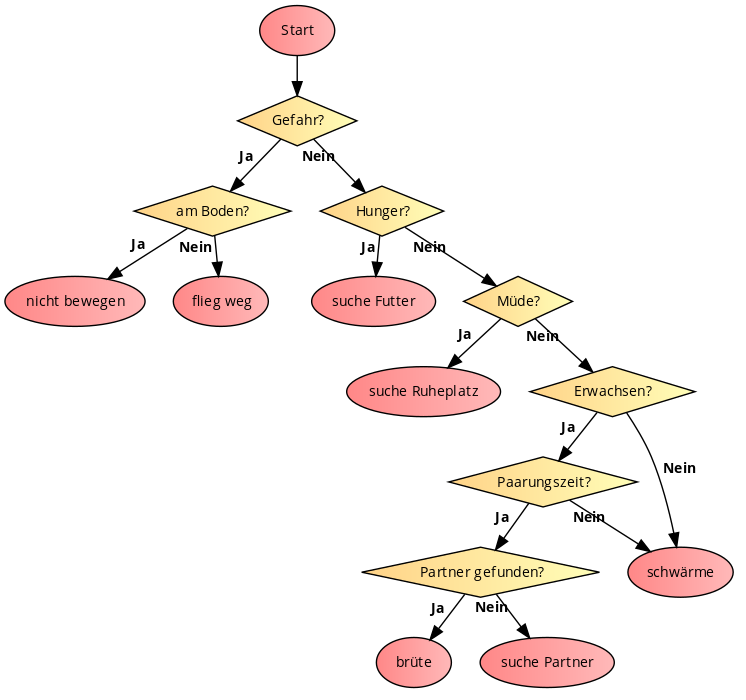
\includegraphics[scale=0.6]{code2flow/entscheidungsfindung.png}
\caption{Entscheidungsfindung}
\label{entscheidung}
\end{figure}

Danach wird entschieden, was der Boid als Nächstes tut. Die Entscheidungssequenz dazu verdeutlicht die Grafik \ref{entscheidung}.

\chapter{Umsetzung}\label{umsetzung}
In diesem Kapitel wird dargestellt, wie das im vorherigen Kapitel entworfene Modell zu einem Prototyp umgesetzt wird. Im ersten Abschnitt findet sich eine Beschreibung der eingesetzten technischen Mittel. Danach folgen die Beschreibung der Architektur, eine Übersicht der Quelldateien, der Ablauf des Prototyps und die Beschreibung der Datenstrukturen der Boids. Abschließend werden die Modellierung der Genetik und Aspekte der Visualisierung behandelt.
\section{Technische Mittel}
In diesem Abschnitt werden die zur Entwicklung eingesetzten technischen Mittel beschrieben.
\subsection{Javascript}
Als Programmiersprache wurde Javascript 6 gewählt. Die Entwicklung mit Javascript ermöglicht ein einfaches Deployment mit einem geeigneten Server. Auch das Testen kann mit einem handelsüblichen Computer, der einen Internetbrowser besitzt, leicht zugänglich gemacht und durchgeführt werden.
\subsection{Server}
Als Webserver wurde lighttp 1.4 gewählt. Dieser Webserver hat eine Open Source Lizenz, ist schnell und einfach zu installieren und bietet vorkonfiguriert das Hosten von HTML- und Javascript-Dateien an. Der Server wurde auf einem handelsüblichen Notebook mit Ubuntu 15.10 64-bit gehostet.
\subsection{Three.js}
Als Grafikbibliothek wurde Three.js (rev. 75) gewählt. Diese Bibliothek besitzt die MIT Lizenz und kann somit für eine Bachelorarbeit benutzt werden. Diese Bibliothek bietet eine umfangreiche Auswahl für die Grafikprogrammierung in 3D mit Javascript an. Es beinhaltet Vektoren, viele primitive Modelle, wie Kugeln, Kameras, Lichtquellen, und eine Render Loop. Die Dokumentation zeigt etliche Beispiele für typische Grafikprobleme.
\subsection{threeoctree.js}
Eine Implementierung von einem dynamischen Octree, threeoctree.js (r60), wurde von Collin Hover für Three.js entwickelt.
\subsection{stats.js}
Für die live Messung der Performanz wurde stats.js gewählt. Diese zeigt sich oben links als kleine Box im Canvas-Bereich des Browsers und liefert aktuelle Messdaten in Form eines Live-Ticker-Balkendiagramms. Es lassen sich durch Mausklick alternativ die FPS (Frames per Second) oder Millisekunden pro Frame anzeigen.
\subsection{Browser}
Als Webbrowser wurde Firefox 47.0 gewählt. Dieser Browser hat eine Open Source Lizenz und ist auf einem aktuellen Ubuntu-System vorinstalliert.
\section{Architektur des Prototyps}
Die Quelldateien werden auf einem Webserver gehostet, die Ausführung der Javascript-Anteile erfolgt aber auf dem Client, der die Adresse des Servers ansteuert.
Die einzelnen Quelldateien und deren Funktionalitäten werden im Folgenden grob erläutert.
\subsection{boids.html}
Dies ist die einzige HTML-Datei des Projektes. Sie stellt den Einstiegspunkt für den Prototyp dar. Hier wird das Browserfenster für den Prototyp vorbereitet: Der ganze Canvas des Browsers wird ausgenutzt, ohne Ränder. Alle anderen Bibliotheken und Quelldateien werden geladen.

Die Live-Messung der Performanz mit stats.js wird gestartet und inital als FPS-Anzeige konfiguriert.
Die Boids werden mit initBoids() initialisiert. Abschließend wird die Render Loop mit renderWorld() gestartet. Diese beiden Methoden befinden sich in den Dateien boids.js und renderer.js.
\subsection{renderer.js}
In dieser Quelldatei befinden sich die Anteile, die sich mit der Grafik beschäftigen. Hier findet sich auch ein EventListener, der die Szene im Fenster neu skaliert, wenn der Browser in seiner Größe verschoben bzw. verzerrt wird. Im Abschnitt Visualisierung \ref{visual} werden die Details erläutert.
\subsection{boids.js}
In dieser Quelldatei finden sich die Modellierung der Boids, die Status-Updates und die Berechnung des Schwärmens. Weitere Details dazu finden sich in den weiteren Abschnitten.
\subsection{helper.js}
Diese Datei beinhaltet Hilfsmethoden. Hier finden sich u.a. Methoden zur zufälligen Generierung von Geschwindigkeit und Geschlecht, sowie die Timer für die Update- und Paarungszeitzyklen.
\subsection{enemy.js}
In dieser Quelldatei wird der Fressfeind bzw. der Angreifer entwickelt. Hier finden sich der Update-Timer des Angreifers, die Details zum Rendering und die Funktionalitäten des Angreifers. Der Angreifer sollte ein getrenntes Modul des Prototyps sein und wird deshalb in eine eigene Quelldatei ausgelagert. Genauere Details zur Implementierung finden sich im Abschnitt Visualisierung \ref{visual}.

\section{Die Render Loop und die Update-Zyklen}
Die Ausführung des Prototyps geschieht in einer Schleife, der Render Loop. Diese Schleife heißt renderWorld() und findet sich in der Quelldatei renderer.js. Hier werden die Performanzmessung mit stats.js erneuert und der aktuelle Zustand der Welt mit den Methoden updateWorld() und updateEnemy() neu berechnet.

Die Methode updateWorld() findet sich in der Quelldatei boids.js. Die Methode updateEnemy() findet sich in der Quelldatei enemy.js.

Danach zeichnet der Renderer die aktualisierte Szene, der Octree wird aktualisiert. Zum Schluss wird mit der Methode requestAnimationFrame(renderWorld) die Schleife wieder neu gestartet. Diese Schleife wird initial gestartet in der boids.html und läuft unendlich weiter, solange der Browser bzw. der Tab des Prototyps geöffnet ist.

\subsection{updateWorld()}
Um die Performanz zu erhöhen, wird die Population nicht in jedem Update-Zyklus aktualisiert, sondern nur in jedem dritten. Dies erschien bei der Entwicklung häufig genug, ohne schnelle Reaktionszeiten der Boids in der Simulation zu verlieren. Die Population wird in der Methode updatePopulationStatus() aktualisiert.

Die aktualisierte Population wird dann ein weiteres Mal aktualisiert. Diesmal werden die Positionen der einzelnen Boids in der Methode updateSwarmingSingle(boid) je nach aktuellem Status neu berechnet.

\subsection{Status der Boids}
Je nachdem, wie die Energiewerte liegen und was der Boid gerade gemacht hat, ändert sich der Status des Boids. Es gibt in dieser Implementierung drei verschiedene Optionen für den Status:
Ein Boid, der gut gesättigt und nicht müde ist, hat üblicherweise den Status "{}SWARMING"{}. Wenn die Energielevel den Schwellwert unterschreiten oder ein adultes Tier sich in der Paarungszeit befindet, so wechselt der Status auf "{}SEARCHINGGROUND"{}. Ein Boid, der sich aus diversen Gründen auf dem Boden aufhält, besitzt den Status "{}ONGROUND"{}.

\subsection{updatePopulationStatus()}
 Hier wird die Population aktualisiert, d.h. alte Boids werden aussortiert. Wenn gerade Paarungszeit ist, werden neue Nachkommen erzeugt. Dabei wird die gesamte Population, d.h. die Boids aus dem Populations-Array, danach überprüft, ob die Boids sich auf dem Boden befinden, und anschließend nach Geschlecht sortiert. Per Zufall werden diese Boids verpaart und ein neues Boidkind erzeugt. Das Erzeugen neuer Boidkinder geschieht in der Methode makeNewBabyBoid(mutter, vater), wie in \ref{babies} beschrieben.

Alle anderen Boids, die nicht verstorben oder neu hinzugefügt worden sind, werden einzeln in der Methode updateSingle(boid) aktualisiert.

\subsection{updateSingle(boid)}
 Hier wird ein einzelner Boid auf seine Energielevel und aktuellen Zustände hin geprüft und angepasst. Zunächst wird abgefragt, ob der Boid auf dem Boden ist. Ist dies der Fall, so wird geprüft, ob der Boid seine Energielevel wieder gefüllt hat. Ist gerade keine Paarungszeit, so erhält der Boid den Status "{}SWARMING"{}. Ist der Boid nicht erholt, so wird der Energielevel weiter angehoben, da sich der Boid ja auf dem Boden befindet und gerade Nahrung aufnimmt.

Ist der Boid nicht auf dem Boden, so werden die Energielevel gesenkt. Ist der Boid müde oder hungrig, so ändert sich der Status auf "{}SEARCHINGGROUND"{}, so dass er jetzt den Boden ansteuern und nach Nahrung suchen kann.
Ist stattdessen Paarungszeit und der Boid ist erwachsen, so sucht der Boid jetzt auch den Boden auf und erhält den Status "{}SEARCHINGGROUND"{}.

\subsection{updateSwarmingSingle(boid)}\label{swarmmethod}
In dieser Methode wird die Position des einzelnen Boids je nach Status neu berechnet. Der zu berechnende Boid überprüft in jedem Fall den Mindestabstand zu seinen Nachbarn. Die Anpassung an Geschwindigkeit und Ausrichtung geschieht allerdings nur, wenn der Boid und der jeweilige Nachbar beide gerade am Schwärmen sind. Sucht der Boid den Boden, so wird der Boid stattdessen nach unten gelenkt.

Ist gerade ein Angreifer in der Nähe, so wird durch Bekanntheit der Position des Angreifers eine geeignete Flucht errechnet. In einer leichtesten Implementierung wird der Angreifer ähnlich der Berechnung des Mindestabstandes als höher priorisierter Nachbar behandelt. Der Boid ist dann zwar auf der Flucht, sucht aber immer noch den Zusammenhalt mit seinen Artgenossen.

Bei der Implementierung fällt auf, dass sich die Boids sehr zitterig hin und her bewegen. Um die Bewegung auszuglätten, wird der neue Bewegungsvektor mit den drei letzten Bewegungsvektoren ausgeglichen.

Die Berechnung des puren Schwärmens richtet sich nach dem mathematischen Modell, welches bereits im Kapitel \ref{mathe} beschrieben wurde.

\section{Datenstrukturen des Schwarms}
Rein theoretisch lässt sich ein Schwarm in einem simplen Array speichern. Aus Performanzgründen ist dies aber nicht empfehlenswert. Auch die Visualisierung benötigt eine eigene Lösung.
\subsection{Struktur des Boid-Objektes}
Die Modellierung der Boids hat in dem Prototyp zwei verschiedene Einsatzzwecke: Einmal als purer, abstrakter Boid, der Teil einer Population ist und Eigenschaften und Bedürfnisse hat; ein anderes Mal als 3D-Objekt, welches von dem Renderer gezeichnet werden muss. Die Trennung von Population und Visualisierung ist zwar wünschenswert, aber leider nicht vollständig möglich, wie weiter unten beschrieben wird \ref{visualstruktur}.

Ein Boid in dem Populations-Array besitzt zunächst die Position, den aktuellen Bewegungsvektor und die Liste der letzten drei Bewegungsvektoren. Dieses sind die drei Informationen, die eine Minimalimplementierung nur für das pure Schwärmen benötigt. In der Methode updateSwarmingSingle(boid) \ref{swarmmethod}, die das Schwärmen der einzelnen Boids berechnet, wird von diesen Informationen Gebrauch gemacht.

Um die Population darzustellen, werden die Informationen über Status und aktuelle Energielevel benötigt. Zur Vererbung sind Genotyp und Phänotyp wichtig. Diese werden in der Struktur der Boids als "{}echter"{} Boid-Anteil gekapselt. Ein Boid hat also in erster Linie bloße Schwärminformationen, besitzt aber einen Erweiterungsteil in Form eines inneren Boids, der dem Populationsgedanken folgt.

Dieser innere Boid besitzt Methoden, die Auskunft geben über die aktuellen Zustände: Das Alter, ob der Boid Hunger hat oder müde ist oder aber gut gesättigt und erholt. Außerdem gibt es Methoden, die Auskunft geben, ob der Boid erwachsen ist oder seine maximale Lebenszeit erreicht hat. Die Energielevel Nahrungsvorrat und Leistungsfähigkeit sowie der aktuelle Status, initial mit "{}SWARMING"{} belegt, sind als Attribute des inneren Boids implementiert.
\subsection{Dynamischer Octree}

\begin{figure}[!h]
\centering
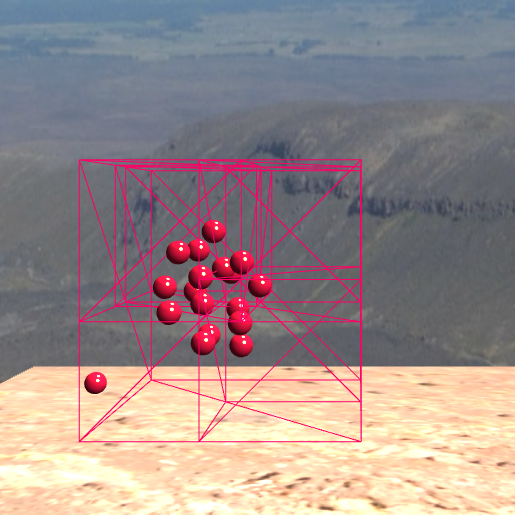
\includegraphics[scale=0.4]{project/octree.png}
\caption{Boids in einem dynamischen Octree}
\label{octree}
\end{figure}

Eine beliebte Variante ist es, eine Datenstruktur zur räumlichen Aufteilung zu wählen \cite{journals/cie/SilvaLC09}\cite{GPGPUFlock13}\cite{214}.
Als Datenstruktur bietet sich im dreidimensionalen Raum ein Octree an. Ein Octree teilt den Raum rekursiv in acht gleichgroße Würfel auf, wobei jeder Würfel wiederum in acht Würfel geteilt werden kann. Ein Octree ähnelt einer Baumstruktur und speichert die Elemente anhand ihrer Position. Da sich die Boids bewegen, müssen die Elemente verschoben werden können. Es wird also eine Struktur benötigt, die mit vielen beweglichen Elementen umgehen kann. Eine solche Struktur ist der dynamische Octree. Die Bibliothek threeoctree.js ist eine Implementierung eines dynamischen Octrees und wurde für den Einsatz mit Three.js entwickelt.

Die Abbildung \ref{octree} visualisiert die Boids in einem Octree, der sich ständig neu aufbaut, um die Positionen der Boids aktuell zu halten.

\subsection{Datenstruktur für die Visualisierung}\label{visualstruktur}
Die Szene speichert sich alle Szenenobjekte intern. Wäre der Schwarm statisch, wäre es genug, alle Mesh-Objekte der Boids der Szene zu übergeben. Nun sind die Boids aber ständig in Bewegung, was die Speicherung des Schwarms in einem eigenen Array erforderlich macht.

In jedem Schwarm-Update wird über die gesamte Population iteriert und deren neue Positionen berechnet. Es gibt also ein Array, das Populations-Array, in dem alle Boids gespeichert werden. Außerdem gibt es ein Array, in dem die Meshes der Boids gespeichert werden. Diese Meshes sind verlinkt mit denen, die der Szene bekannt sind. In der Methode addBoidToSzene(boid) in der Quelldatei renderer.js wird der neu angelegte Boid an ein neues Mesh übergeben. Dieses Mesh wird zu dem Mesh-Array und der Szene hinzugefügt. Da für das Finden der nächsten Nachbarn ein Octree existiert, wird das Mesh an dieser Stelle auch dem Octree bekannt gemacht.

Um ein Boid wieder aus der Szene zu entfernen, muss zunächst der richtige Boid ausfindig gemacht werden. Eine eindeutige Indentifikation erfolgt über die Angabe des Geburtstages. Dazu wird das THREE.Mesh erweitert. Das Mesh-Array wird in der Methode removeBoidFromSzene(boid) nach dem Geburtstag durchsucht. Das gefundene Objekt ist das Mesh-Objekt des zu entfernenden Boids. Sowohl die Szene als auch der Octree besitzen Methoden zum Entfernen von Szenenobjekten, in denen lediglich das zu entfernende Objekt übergeben werden muss.

\section{Genetik}
Die Modellierung der Boids und deren Erbgut findet sich in der Quelldatei boids.js. In diesem Abschnitt werden die Einzelheiten zu der Genetik, dem initialen Generieren der Ursprungspopulation und der Vererbung des Erbguts an Nachkommen beschrieben.

\subsection{Genotyp}
Der Genotyp beinhaltet das Erbgut. Jede Eigenschaft bzw. jedes Gen hat zwei Optionen: eine von dem Vatertier und eine von dem Muttertier. Der Genotyp der Boids in diesem Prototyp speichert die folgenden Eigenschaften: die Lebensspanne, die maximale Ausdauerkapazität, die maximale Beschleunigungskraft, die Höchstgeschwindigkeit, das Geschlecht und die Zeit der Geschlechtsreife. Die initialen Werte, die die Boids in dem Prototyp erhalten, sind in der Tabelle \ref{genotyp} aufgelistet.

\begin{table}[!h]
\centering
\begin{tabular}{l|c|c}
	Gen & Option 1 & Option 2\\
	\hline
	Lebensspanne & 30 000 & 60 000\\
	Maximale Ausdauer & 100 & 200\\
	Nahrungskapazität & 30 & 50\\
  Maximale Beschleunigungskraft & 0.4 & 0.6\\
  Maximale Geschwindigkeit & 2 & 4\\
  Geschlecht & m & w\\
  Geschlechtsreife & 180 & 300\\
\end{tabular}
\caption{Initiale Werte des Genotyps}
\label{genotyp}
\end{table}

\subsection{Phänotyp}
Der Phänotyp beinhaltet die tatsächliche Ausprägung des Genotyps und wird in der Methode calcPhenotype(genotype) anhand des vererbten Genotyps erstellt. Hier wird für jedes Gen bzw. jede Eigenschaft zufällig eine von beiden vorhandenen Optionen ausgewählt. Zusätzlich enthält der Phänotyp den Geburtstag des Boids, welcher bei diesem Prototyp einfach der Timestamp der Erzeugung des Boids ist. Alle Handlungen und Berechnungen finden auf Basis des Phänotyps statt.

\subsection{Initiale Generierung der Boids}
Beim Starten des Prototyps muss zuerst ein neuer Schwarm generiert werden. Dies erfolgt in der Methode initBoids(anzahl). Die Hilfsmethode addRandomBoid() erzeugt einen zufälligen neuen Boid. Der Genotyp wird dabei in der Methode initGenotype() zufällig erzeugt. Hier werden die für die Simulation benötigten Parameter mit fast zufälligen Werten belegt. Fast bedeutet, dass Bereiche für die Werte vorprogrammiert werden.

\subsection{makeNewBabyBoid(muttertier, vatertier)}\label{babies}
Die Erzeugung eines neuen Boidkindes verläuft ähnlich wie die Erzeugung eines initial, zufällig generierten Boids. Der Unterschied liegt in der Erzeugung des Genotyps. Wenn ein Nachkomme erzeugt wird von bereits existierenden Eltern, dann muss der Genotyp von den Elterntieren abhängen. Die Methode genSplicer(mum.boid.genotype, dad.boid.genotype) erzeugt einen neuen Genotyp, indem für jedes Gen zufällig eine Option des gleichen Genes von dem Muttertier und eine Option von dem Vatertier ausgewählt wird.

\section{Visualisierung}\label{visual}
Die Visualisierung zeigt eine Population von Boids. Die Visualisierung beschränkt sich auf das Nötigste, da die Umsetzung der Funktionalitäten höhere Priorisierung hat.
Die Entitäten, die sich mit dem Rendering beschäftigen, sind, sofern nicht anders angegeben, Teil der Three.js-Bibliothek.

\subsection{Szenario}
Das Szenario der Visualisierung beinhaltet eine kleine Gruppe von 20 Boids, die ohne Einfluss oder Skripte über den Bildschirm schwärmt und dabei in regelmäßigen Abständen Mitglieder verliert oder dazugewinnt oder deren Mitglieder wie in der Abbildung \ref{swarming} zur Nahrungsaufnahme den Boden aufsuchen. Des Weiteren erscheint ab und zu ein Fressfeind, dem die Boids entkommen müssen.

\begin{figure}[!h]
\centering
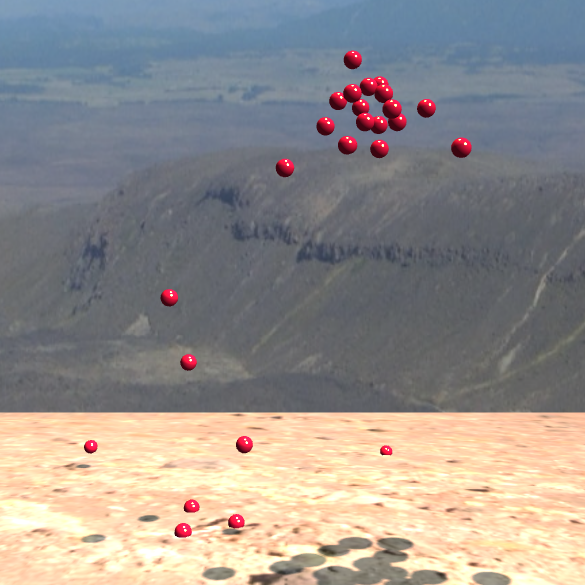
\includegraphics[scale=0.4]{project/upheaval.png}
\caption{Ein Schwarm von Boids mit unterschiedlichen Bestrebungen}
\label{swarming}
\end{figure}

\subsection{Visualisierung der Boids}
Ein grundlegendes Merkmal von Schwarmtieren ist das homogene Erscheinungsbild. Eine Visualisierung, die Anspruch auf Realitätsnähe erheben möchte, muss die Boids demnach zwingend identischen Aussehens realisieren. In dem Prototyp wurden die Boids deshalb alle als Kugeln in derselben Größe und Farbe dargestellt. Der Einsatz eines komplexeren 3D-Modells wurde bewusst nicht gewählt, da so das Verhalten der Boids im Vordergrund bleiben kann. In der Quelldatei renderer.js werden die 3D-Modelle der Boids angelegt. Jeder Boid ist eine einfache Kugel, eine SphereGeometry, und kann mit dem Attribute castShadow auf true gesetzt Schatten werfen.

\subsection{Darstellung der Szene}
Die Szene ist sehr einfach gehalten. Optisch ansprechende Details, wie z.B. Bäume, hätten die Szene zwar schöner dargestellt, wären aber Hindernisse, die die Boids hätten umgehen müssen. Da der Schwerpunkt dieser Arbeit auf dem Populationsgedanken liegt und nicht auf dem Navigieren auf einem komplexen Terrain, wurde davon Abstand genommen. Alle Anteile der Szenendarstellung finden sich in der Quelldatei renderer.js.

Zunächst wird der WebGLRenderer geladen. Im Gegensatz zu anderen ist dieser Renderer in der Lage, direkt auf die Grafikkarte zuzugreifen. Es handelt sich bei WebGL um eine Implementierung des sehr populären OpenGLs. Der Renderer wird auf die gesamte Größe des Browserfensters skaliert und die Shadow Map des Renderers wird auf enabled gesetzt, damit die Szene durch das Rendering von Licht und Schatten plastischer wirken kann.

Die Szene wird gestartet und eine PerspectiveCamera auf die Position (x: 50, y: 100, z: 300) gesetzt. Sie ist auf den Mittelpunkt der Bodenfläche (x: 0, y: -100, z: 0) ausgerichtet. Diese Position ermöglicht es dem Betrachter, den Großteil der Szene und damit des Geschehens im Auge zu behalten.

Als Nächstes werden zur angenehmen Beleuchtung eine ambiente Lichtquelle sowie ein Spotlight initialisiert. Letzteres sorgt durch das Setzen des Attributes castShadow auf true dafür, dass die Boids in der Szene Schatten werfen können. Die Position des Spotlights (x: 20, y: 200, z: 20) wird oberhalb der Szene gesetzt. Das Ziel seiner Ausrichtung ist ebenfalls, wie das der Kamera, der Mittelpunkt des Bodens.

Auch ein einfacher Hintergrund wird geladen. Als Asset dient hier eine Photografie einer Landschaft. Der einzige Zweck ist die optische Abgrenzung der Szene. Geladen wird das Asset mit dem TextureLoader und als Textur auf eine Ebene projiziert.

Der Boden wird durch einen sehr flachen Quader modelliert. Er befindet sich am unteren Ende der Bounding Box \ref{box}. Mit dem Setzen des Attributes receiveShadow auf true ist der Boden in der Lage, Schatten, die durch die Boids geworfen werden, zu zeigen.

\subsection{Animation des Fressfeindes}
Damit die Boids das Verhalten einem Angreifer gegenüber zeigen können, wird ein solcher selbstverständlich in der Szene benötigt. Da in erster Linie die Boids für dieses Modell interessant sind und nicht der Fressfeind, wurde dieser nur rudimentär umgesetzt. Der Fressfeind ist, wie die Boids auch, eine einfache Kugel, die sich allerdings in Größe und Farbe unterscheidet, wie das ja auch in der Natur der Fall wäre. Der Fressfeind in dem Prototyp ist nicht mit eigener Intelligenz ausgestattet, er durchstreift lediglich in periodischen Abständen die Szene. Abbildung \ref{enemy} zeigt den Fressfeind in Aktion.

\begin{figure}[!h]
\centering
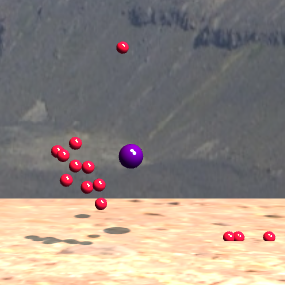
\includegraphics[scale=0.8]{project/enemy.png}
\caption{Ein Schwarm von Boids wird angegriffen.}
\label{enemy}
\end{figure}

Die Boids überprüfen in ihren Update-Zyklen, wie bereits \ref{swarmmethod} beschrieben, ob und wo sich der Fressfeind befindet, um ihm dann bei zu geringer Distanz auszuweichen. Dieser Ansatz folgt der zweiten Strategie wie oben \ref{enemy} bereits beschrieben.
\subsection{Begrenzung der Szene}\label{box}
Damit die Boids nicht aus dem Sichtfeld der Szene entschwinden, wird eine Bounding Box, also eine Begrenzung des Raumes, eingesetzt. Die Modellierung der Bounding Box als Würfel erscheint als die einfachste Möglichkeit, wobei der Mittelpunkt der Bounding Box dem Mittelpunkt des Koordinatensystems der Szene entspricht. Dies ermöglicht die einfache Erkennung, wann ein Boid Gefahr läuft, die Bounding Box zu verlassen. Nach der Berechnung der neuen Position eines Boids werden alle Koordinaten dieser Position daraufhin geprüft, ob der Absolutwert einer Koordinate größer als die halbe Seitenlänge der Bounding Box ist. Ist dies der Fall, so hat der Boid die Grenze erreicht. Um zu verhindern, dass der Boid diese Grenze tatsächlich überschreitet, wird der Wert der überschreitenden Koordinate auf den Grenzwert beschränkt. Die Vektoren der Three.js Bibliothek bieten dazu die Methode clamp(vector1, vector2), mit vector1 = (-r,-r,-r) und vector2 = (r,r,r), wobei r die halbe Seitenlänge der Bounding Box ist. In diesem Prototyp wurde r = 100 festgelegt.

\chapter{Evaluation}\label{eval}
In diesem Kapitel werden das in Kapitel \ref{modell} entworfene Modell und der nach diesem Modell entwickelte Prototyp, der in Kapitel \ref{umsetzung} beschrieben wird, evaluiert. Da der Ansatz dieser Arbeit sich auf populationstypische Kriterien fokussiert, wird als Erstes untersucht, wie stabil die Boids-Population ist, wie sich der Genpool verändert und welche Ursachen das haben könnte. Im Anschluss daran werden kurz Eindrücke zur Performanz der Simulation beschrieben, die während der Umsetzung des Prototyps aufgefallen und Schwierigkeiten bereitet haben.

\section{Populationsdynamik}
\begin{figure}[h]
\centering
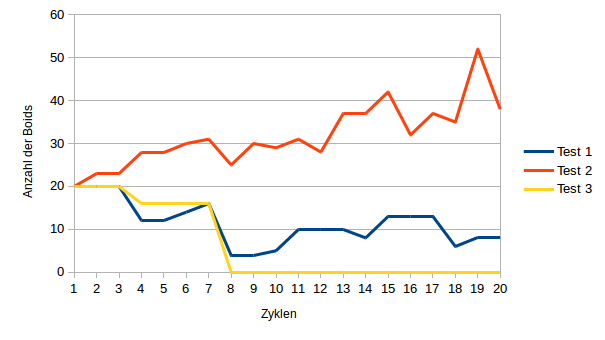
\includegraphics[scale=0.8]{project/Test1-Populationen.png}
\caption{Verlauf der Populationsfluktuation bei drei Testläufen}
\label{populationsgrafik}
\end{figure}

Die Stabilität einer Population erkennt man anhand der Geburten- und Sterberate. Dazu wird die Population des Prototyps gestartet und beobachtet, indem alle 500 Zyklen die Populationsgröße gemessen wird. Um die Stabilität genauer untersuchen zu können, werden außerdem die Anzahl der Geburten und die Anzahl der Todesfälle getrennt ermittelt. Um die Population isoliert zu testen, wird auf den Einfluss von Fressfeinden verzichtet. Auch das Angebot von Nahrung wird ausreichend gestaltet.

Insgesamt werden zum Start 20 Zyklen mit 20 Boids gemessen und der Test dreimal durchgeführt.

Wie in der Grafik \ref{populationsgrafik}, die die Populationsgrößen zeigt, zu erkennen ist, weichen die drei Testläufe stark voneinander ab. Der erste Testlauf unterliegt großen Schwankungen und hat nie mehr Boids als die anfänglichen 20. Die Population im zweiten Testlauf hingegen ist teilweise auf mehr als das Doppelte angewachsen. Der dritte Testlauf verliert bereits nach dem siebten Zyklus alle Schwarmtiere.

Die einzelnen Details zeigen die folgenden Tabellen. Die Tabellen zeigen nur die Zyklen, in denen es eine Veränderung gab.

\begin{table}[!h]
\centering
\begin{tabular}{c|c|c|c|c|c}
	Zyklus & Populationsgröße & Weibchen & Männchen & Anz. d. Geburten & Anz. d. Todesfälle\\
	\hline
	1 & 20 & 7 & 13 & 0 & 0\\
	4 & 12 & 4 & 8 & 0 & 8\\
	6 & 14 & 5 & 9 & 2 & 0\\
	7 & 16 & 7 & 9 & 2 & 0\\
	8 & 4 & 3 & 1 & 0 & 12\\
	10 & 5 & 3 & 2 & 2 & 1\\
	11 & 10 & 5 & 5 & 5 & 0\\
	14 & 8 & 3 & 5 & 2 & 4\\
	15 & 13 & 4 & 9 & 5 & 0\\
	18 & 6 & 2 & 4 & 0 & 7\\
	19 & 8 & 3 & 5 & 2 & 0\\
\end{tabular}
\caption{Test 1 zur Populationsdynamik}
\label{dynamik1}
\end{table}

Den ersten Testverlauf visualisiert die Tabelle \ref{dynamik1}.
Auffällig ist das Verhältnis zwischen den Geschlechtern, meistens sind die Männchen deutlich in der Überzahl. Nur im achten Zyklus ist dies nicht so. Dort ist die Population mit nur vier Boids und einem einzelnen Männchen kurz vor dem Aussterben. Trotzdem erholt sich die Population in den nachfolgenden Zyklen.

Ist die Anzahl der Geburten relativ stabil, so zeigt sich bei der Anzahl der Todesfälle doch ein ganz anderes Muster: Entweder sterben keine Boids oder ganz viele gleichzeig. Im achten Zyklus beträgt die Sterberate sogar 75 \%. Außerdem findet dieses Massensterben in regelmäßigen Abständen statt.

\begin{table}[!h]
\centering
\begin{tabular}{c|c|c|c|c|c}
	Zyklus & Populationsgröße & Weibchen & Männchen & Anz. d. Geburten & Anz. d. Todesfälle\\
	\hline
	1 & 20 & 9 & 11 & 0 & 0\\
	2 & 23 & 10 & 13 & 3 & 0\\
	4 & 28 & 12 & 16 & 16 & 11\\
	6 & 30 & 13 & 17 & 4 & 2\\
	7 & 31 & 14 & 17 & 1 & 0\\
	8 & 25 & 15 & 10 & 13 & 19\\
	9 & 30 & 18 & 12 & 5 & 0\\
	10 & 29 & 18 & 11 & 3 & 0\\
	11 & 31 & 18 & 13 & 2 & 0\\
	12 & 28 & 14 & 14 & 12 & 15\\
	13 & 37 & 18 & 19 & 9 & 0\\
	14 & 37 & 18 & 19 & 2 & 2\\
	15 & 42 & 21 & 21 & 5 & 0\\
	16 & 32 & 13 & 19 & 2 & 12\\
	17 & 37 & 15 & 22 & 5 & 0\\
	18 & 35 & 16 & 19 & 3 & 5\\
	19 & 52 & 27 & 25 & 17 & 0\\
	20 & 38 & 23 & 15 & 4 & 18\\
\end{tabular}
\caption{Test 2 zur Populationsdynamik}
\label{dynamik2}
\end{table}

Den zweiten Testverlauf visualisiert die Grafik \ref{dynamik2}. Auch hier zeigt sich ein getaktetes Massensterben. Aber auch die Geburtenrate schwankt gewaltig. Dafür ist im Gegensatz zu dem ersten Testverlauf das Verhältnis zwischen den Geschlechtern ausgewogen.

Die Tabelle des dritten Testlaufes \ref{dynamik3} wird auf die ersten acht Zyklen beschränkt, da die Population im siebten Zyklus verstirbt. Da die Population nur so kurze Zeit existierte, können hier keinerlei bedeutsame Beobachtungen gemacht werden.

\begin{table}[!h]
\centering
\begin{tabular}{c|c|c|c|c|c}
	Zyklus & Populationsgröße & Weibchen & Männchen & Anz. d. Geburten & Anz. d. Todesfälle\\
	\hline
	1 & 20 & 7 & 13 & 0 & 0\\
	4 & 16 & 6 & 10 & 3 & 7\\
	8 & 0 & 0 & 0 & 0 & 16\\
\end{tabular}
\caption{Test 3 zur Populationsdynamik}
\label{dynamik3}
\end{table}

\section{Populationsgenetik}
Zur Untersuchung der Genetik werden beispielhaft zwei Gene ausgesucht, die beobachtet werden: die Lebensspanne und die maximale Geschwindigkeit.
Es wird beim Starten der Population ermittelt, welche Werte im Erbgut der Boids vorhanden sind. Dieser Test wird alle 500 Zyklen wiederholt. Um diesen Test etwas kompakter zu gestalten, werden der Ursprungspopulation feste Werte zum Start übergeben. Wie bei dem Testen zur Populationsdynamik wird die Population isoliert betrachtet.

Als Anfangswerte werden 30 000 ms bzw. 60 000 ms für die Lebensspanne sowie 2.5 bzw. 3.5 als Werte der maximalen Geschwindigkeit gegeben. Insgesamt werden 20 Zyklen mit 20 Boids zum Start gemessen und der Test dreimal durchgeführt.

Da es sich um die gleichen Testläufe handelt wie bei der Populationsdynamik, kann man dadurch Rückschlüsse auf die Wechselwirkungen zwischen Populationsbestand und genetischer Vielfalt ziehen.

\begin{figure}[!h]
\centering
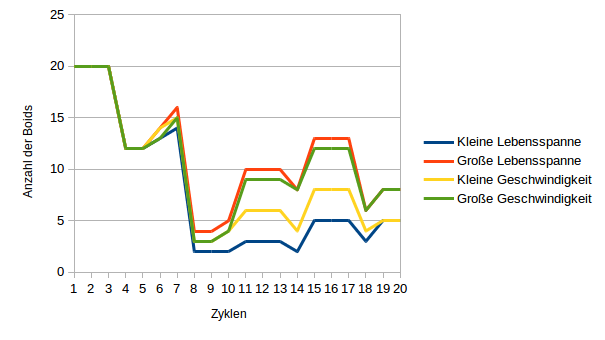
\includegraphics[scale=0.80]{project/Test1-Genetik.png}
\caption{Test 1 zur Distribution der genetischen Varianz}
\label{test1genetik}
\end{figure}

Umso erstaunlicher ist das Ergebnis des ersten Testlaufes. In der Grafik \ref{test1genetik} wird gezeigt, wieviele Boids die jeweilige Option des jeweiligen Gens in ihrem Erbgut tragen. Ob ein Boid dabei nur eine Option doppelt oder beide in seinem Erbgut besitzt, wird hier nicht explizit deutlich.

Obwohl die Population im gesamten Verlauf des Testes so wenige Boids hat und zwischendurch im achten Zyklus fast vor dem Aussterben ist, gibt es am Ende des Tests noch sehr viele Boids, die beide Optionen im Erbgut tragen und so die genetische Varianz sicherstellen.

\begin{figure}[!h]
\centering
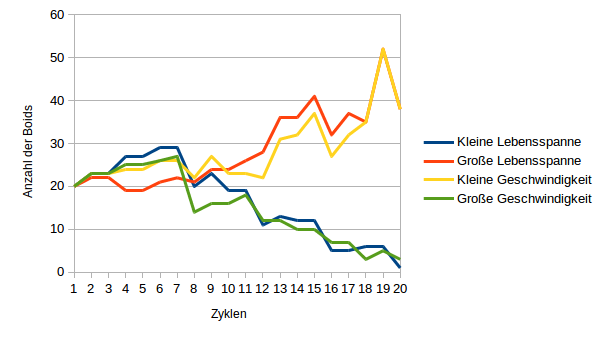
\includegraphics[scale=0.80]{project/Test2-Genetik.png}
\caption{Test 2 zur Distribution der genetischen Varianz}
\label{test2genetik}
\end{figure}

Im zweiten Testlauf hingegen zeigt sich jedoch ein ganz anderes Muster, wie in der Grafik \ref{test2genetik} zu sehen ist. Hier ist deutlich ersichtlich, dass die längere Lebensspanne und die maximale Geschwindigkeit anfangen, sich im Erbgut der Population durchzusetzen. Zum Ende des Tests sind die anderen Optionen fast verschwunden. Die genetische Vielfalt ist trotz der großen Anzahl der Boids sehr gering.

Die Population des dritten Testlaufes, zu sehen in Grafik \ref{test3genetik}, stirbt aus, bevor sich in dem Erbgut Muster zeigen können.

\begin{figure}[!h]
\centering
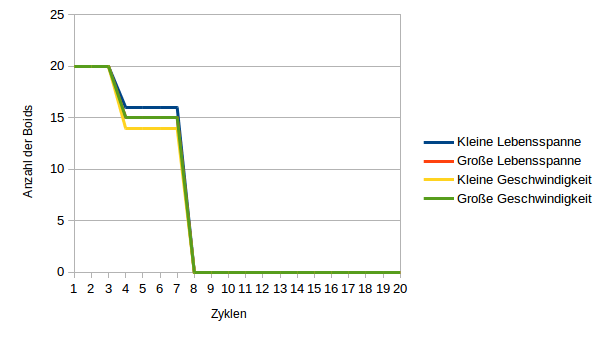
\includegraphics[scale=0.80]{project/Test3-Genetik.png}
\caption{Test 3 zur Distribution der genetischen Varianz}
\label{test3genetik}
\end{figure}

\section{Ursachenforschung}
Eine große Schwierigkeit bei der Entwicklung des Prototyps ist die Ausbalancierung der Parameter. Dauert eine Paarungszeit zu lange, so explodiert die Population, ist die Paarungszeit zu kurz, so bleibt den Boids nicht genügend Zeit, den Boden aufzusuchen und dort einen Paarungspartner zu finden. Werden die Boids zu alt, ist die Sterberate zu gering. Ist der Schwellwert der Energiewerte zu niedrig, so bleibt den Boids nicht genügend Zeit, den Boden zu erreichen, besonders wenn die maximale Geschwindigkeit zu gering dafür ist. Gleichzeitig sollen alle Phasen der Simulation für den Beobachter erkennbar sein. Zwischendurch muss der Schwarm auch wieder Gelegenheit haben zu schwärmen. Auch dies benötigt Zeit, da sich die einzelnen Boids nach Aktivitäten wie Nahrungsaufnahme und Paaren erst wieder finden müssen.

Diese Schwierigkeit, eine Population stabil zu halten, ist in den Testläufen mehr als deutlich zu erkennen. Dies ist aber nicht unbedingt etwas Negatives. Denn auch in der Natur finden sich vielfältige Populationsverläufe, die von deutlich mehr Faktoren abhängen, als es bei den Boids in diesem Prototyp der Fall ist.

Das Muster in der Sterberate erklärt sich, wenn man bedenkt, dass die Tiere ja alle gleichzeitig geboren werden und in dem Test nur zwei mögliche Lebensspannen haben. Würde man den Test mit zufälligen Lebensspannen starten, hätte man weniger Massensterben.

\section{Performanz}
Die Performanz hat großen Einfluss auf die Ästhetik einer Schwarmsimulation. Je größer die Anzahl der Schwarmtiere, desto imposanter wirkt die Simulation. Gleichzeitig gilt aber auch, dass die Performanz sinkt, wenn die Anzahl der Schwarmtiere größer wird. Der originale Algorithmus hat dabei die geringste Performanz, wie bereits in Kapitel \ref{lahm} beschrieben wird. Die Wahl einer Datenstruktur kann hier Verbesserungen bringen. Die räumliche Aufteilung mithilfe eines Octrees erscheint logisch, besonders wenn der Octree mit bewegten Objekten umgehen kann. Dennoch bringt der Octree nur geringe Leistungsverbesserungen, denn der Algorithmus des Schwärmens beinhaltet nicht nur die Berechnung des Schwärmens, sondern auch noch die anderen Update-Zyklen, in denen wiederholt Iterationen über die gesamte Population nötig sind.

Zuerst wird über die Population iteriert, um die alten Boids auszusortieren. Bei der Aussortierung muss im schlimmsten Fall der ganze Schwarm zur Identifikation der zu entfernenden Boids gefiltert werden. Dann wird ein zweites Mal über die Population iteriert, um die Energielevel der übrig gebliebenen Boids und deren Status zu aktualisieren. Wenn Paarungszeit ist, wird die Population nach Boids gefiltert, die auf Partnersuche sind. Abschließend wird die Population ein weiteres Mal durchlaufen, diesmal zur Neuberechnung des Schwärmens. Nur im letzten Durchlauf kann eine Änderung der räumlichen Datenstruktur greifen. Zumindest die ersten beiden Iterationen können, wie in der Umsetzung bereits geschehen, zusammengefasst werden und gemeinsam ablaufen.

Abgesehen von den Algorithmen gibt es noch andere langsame Vorgänge. So muss der Octree häufig aktualisiert werden, um die bewegten Objekte aktuell zu halten. Die jedoch langsamste Aktivität ist das Rendering. Auch wenn in dem Prototyp WebGL verwendet wird, bleibt dies ein Bottleneck. Eine Verringerung der Update-Zyklen reduziert das ständige Neuberechnen und lässt die Simulation weniger stottern. Trotzdem dauert die Berechnung noch sehr lange und führt zu sehr niedrigen Framerates.

\section{Sichtbarkeit}
Die Auswahl der dichtesten Nachbarn erfolgt in dem Prototyp über einen Octree, der diese Nachbarn in einem gegebenen Radius sucht. Je nachdem, wieviele Boids sich gerade in diesem Radius befinden, werden mal mehr und mal weniger Nachbarn gefunden.

Dies bedeutet, dass sich auch immer wieder zwischendurch einzelne Boids zeigen, die den Anschluss an den Schwarm verlieren, weil sie zwischendurch den Boden aufsuchen und der Rest des Schwarmes sich aus ihrer Reichweite entfernt. Diese Boids warten dann so lange, bis der Schwarm zufällig wieder in Reichweite vorbeifliegt. Solche verlassenen Tiere hätten in der Natur geringe Lebenschancen.

Wie bereits in Kapitel \ref{natur} beschrieben, erfolgt die Auswahl in echten Schwärmen aus topologischer Sicht, die zudem noch anisotrop ist. In einer erneuten Umsetzung sollte ein Boid also besser eine variablere Reichweite haben. Dazu könnte man den Octree nutzen, indem man in immer größer werdenden Radien sucht, bis man die gewünschte Anzahl an Nachbarn hat.

Ein anderer Ansatz modelliert das Sichtfeld der Boids mithilfe von Visibility Culling \cite{journals/cie/SilvaLC09}. Diese Methode findet auch weiter entfernte Tiere und kann anisotrop umgesetzt werden.

\chapter{Ausblick und Fazit}\label{fazit}
In diesem Kapitel werden die Arbeit zusammengefasst und einige Weiterentwicklungsmöglichkeiten angesprochen. Den Abschluss bildet ein kurzes Fazit.
\section{Zusammenfassung}
In dieser Arbeit wird ein Modell entwickelt, welches eine Simulation von Schwarmtieren um populationstypische Eigenschaften erweitert. Dazu wird zunächst ein Einblick in die Vorbilder der Natur, verschiedene Methoden der Schwarmsimulation sowie die Grundlagen des Boids-Modells gegeben. Danach wird ein Modell entwickelt, welches auf dem Boids-Modell beruht und zusätzlich um populationstypische Elemente erweitert wird. Anhand dieses Modells wird ein Prototyp entwickelt, welcher das erweiterte Populationsmodell umsetzt. Im Anschluss wird die Evaluation des Prototyps beschrieben.
\section{Weiterentwicklungsmöglichkeiten}
Das in dieser Arbeit beschriebene Modell zeigt einen ersten Ansatz zur Darstellung einer Schwarmpopulation. Möglichkeiten zur Weiterentwicklung bieten sich an.
\subsection{Visualisierung}
Zunächst gibt es Potential für die Visualisierung, sei es in Form von ansprechenden 3D-Modellen für die Boids und der anderen Assets oder Animationsequenzen für wichtige Ereignisse. So könnte ein Boid, der in der Luft verstirbt, zunächst einmal in Richtung Boden fallen, bevor der Boid aus der Szene eliminiert wird.

\subsection{Performanz}
Wie im Kapitel \ref{eval} beschrieben, lässt die Performanz des Prototyps noch deutlich Verbesserungen zu. Eine Optimierung der Datenstrukturen kann hier angestrebt werden.

Da das Rendering durch das Aktualisieren und Neuberechnen des Schwarms stark verlangsamt wird und schnell ins Stocken gerät, d.h. die Framerate stark sinken lässt, wäre eine Umsetzung auf Delta Time Rendering zu untersuchen.

\subsection{Populationsdynamik}
Das Modell kann noch um populationstypische Elemente erweitert werden. Die Natur liefert zahlreiche Beispiele. Eine Möglichkeit wäre es, die Futtersuche komplexer zu gestalten. In dem jetzigen Modell finden die Boids immer ausreichend Nahrung auf dem Boden, egal wo sie sich gerade befinden. Hier könnte man das Szenario realitätsnäher gestalten und ausgewählte Futterstellen modellieren, die erst gefunden werden müssen.

Auch intelligentere Fressfeinde, Verdrängen durch andere Populationen oder Naturkatastrophen bieten noch viel Potential.

Des Weiteren können die Parameter, die die Phasen der Abläufe oder der Eigenschaften der Boids bestimmen, mithilfe von genetischen Algorithmen optimiert werden. Hierzu gibt es bereits einige Ansätze \cite{sab92:reynolds}\cite{oai:CiteSeerXPSU:10.1.1.61.9858}\cite{conf/ecms/AlaliyatYS14}, die dazu untersucht werden können.

\subsection{Populationsgenetik}
Schlussendlich bietet auch die Vererbung Weiterentwicklungsmöglichkeiten: Bei der Rekombination der Gene fehlt z.B. noch die Möglichkeit der Mutation. Außerdem könnten die Boids z.B. die Monogamie und damit einen festen Partner fürs Leben wählen.

Die Partnersuche insgesamt ist noch sehr rudimentär in dem Prototyp entwickelt worden. Das Brüten findet praktisch noch gar nicht statt, die Boidkinder sind sofort flügge und unabhängig von den Elterntieren. Ein längeres Verweilen am Nest, wobei sich die Partner bei der Futtersuche abwechseln, und die Versorgung der Jungtiere sind nur einige mögliche Szenarien, die weiter ausgestaltet werden können.

\section{Fazit}
Das in dieser Arbeit entwickelte Modell zeigt, wie das einfache Boids-Modell in eine Population umgewandelt werden kann. Die Populationsforschung im Kapitel \ref{eval} hat gezeigt, wie komplex und unberechenbar und damit abwechslungsreich eine Simulation mit den Boids sein kann.

Außerdem zeigt sich, dass für eine ansprechende Simulation auch noch andere Faktoren, wie z.B die Performanz, einen nicht unerheblichen Aufwand erfordern.

Abschließend ist dieses Modell ein Einstieg, der wesentliche Bereiche einer Population von Schwarmtieren beinhaltet, wenngleich es noch viel Potential für Weiterentwicklungen gibt.

%%%%

%% appendix if used
%%\appendix
%%\typeout{===== File: appendix}
%%\include{appendix}

% bibliography and other stuff
\backmatter

%%\nocite{*}
\typeout{===== Section: literature}
%% read the documentation for customizing the style
\bibliographystyle{plain}
\bibliography{boids}

\typeout{===== Section: nomenclature}
%% uncomment if a TOC entry is needed
%%\addcontentsline{toc}{chapter}{Glossar}
\renewcommand{\nomname}{Glossar}
\clearpage
\markboth{\nomname}{\nomname} %% see nomencl doc, page 9, section 4.1
\printnomenclature

%% index
\typeout{===== Section: index}
\printindex

\HAWasurency

\end{document}
\grid
\grid
\grid
\grid
\grid
\grid
\grid
\grid
\grid
\grid
\grid
\grid
